\documentclass[specialist, 12pt,
subf, %draft,
href, colorlinks=true,
substylefile = spbu.rtx,
]{disser}

%draft
\usepackage[
a4paper, mag=1000, includefoot,
left=3cm, right=1.5cm, top=2cm, bottom=2cm, headsep=1cm, footskip=1cm
]{geometry}

\usepackage{float}
\usepackage[T2A]{fontenc}
\usepackage[utf8]{inputenc}
\usepackage[english,russian]{babel}
\ifpdf\usepackage{epstopdf}\fi
\usepackage{cmap}
\usepackage{graphicx}
\usepackage{multicol,caption}
\usepackage[final]{listings}
\usepackage[ruled,linesnumbered]{algorithm2e}
\usepackage{amsmath}
\usepackage{amsthm}
\usepackage{amssymb}
\usepackage{amsfonts}
\usepackage{listings}
\usepackage{xcolor}
\usepackage{wrapfig}
%\usepackage{subfigure}
%\usepackage{longtable}
\usepackage{array}
%\usepackage{bbold}
\usepackage{subcaption}
\setcounter{MaxMatrixCols}{48}
\usepackage{resizegather}
\usepackage{hyperref}
\let\vec=\mathbf
\widowpenalty=10000
\clubpenalty=10000
\setcounter{tocdepth}{2}

\usepackage{bm}

\makeatletter %%%%% <---- Starting chapter without a pagebreak
\renewcommand\chapter{\par%
\thispagestyle{plain}% \global\@topnum\z@
\@afterindentfalse \secdef\@chapter\@schapter}
\makeatother %%%%% <---- Starting chapter without a pagebreak

\graphicspath{{imgPCA/}}


\newtheorem{proposition}{Предложение}
\newtheorem{definition}{Определение}
\newtheorem{theorem}{Теорема}
\newtheorem{investigation}{Следствие}
\newtheorem{designation}{Обозначение}
\newtheorem{remark}{Замечание}
\newtheorem{example}{Пример}

\DeclareMathOperator{\diag}{diag}
\DeclareMathOperator{\spn}{span}
\DeclareMathOperator{\rnk}{rank}
\DeclareMathOperator{\dist}{dist}
\begin{document}
	
	\lstset{
		basicstyle=\ttfamily\footnotesize, % the size of the fonts that are used for the code
		numbers=left, % where to put the line-numbers
		numberstyle=\footnotesize, % the size of the fonts that are used for the line-numbers
		stepnumber=1, % the step between two line-numbers. If it's 1, each line
		% will be numbered
		numbersep=8pt, % how far the line-numbers are from the code
		language=R}
	\institution{
		Санкт-Петербургский государственный университет \\
		Прикладная математика и информатика \\
		Статистическое моделирование
	}
	
	
	\author{Лекции Голяндиной Нины Эдуардовны для магистров первого курса\thanks{Первоначальный набор: Третьякова Александра, Зенкова Наталья}}
	
	% Тема
	\title{{\normalfont\scshape
	Многомерный анализ данных: SVD, PCA, FA}\\
Черновой вариант, просьба сообщать об опечатках}
	
	% Автор


	
	% Город и год
	\city{Санкт-Петербург}
	\date{\today}
	
	
	
	\maketitle
	\tableofcontents
	
	\intro
	\section{Генеральный язык} \label{q2}
Пусть случайная величина $\bm\xi = (\xi_1, \ldots, \xi_p)^{\mathrm{T}} \in \mathbb{R}^p$, где $p$ --- количество признаков. Обозначим
\begin{itemize}
	\item \textit{вектор средних} $\bm\mu = (\textsf{E}\xi_1, \ldots, \textsf{E}\xi_p)^{\mathrm{T}} \in \mathbb{R}^p$;
	\item \textit{ковариационную матрицу} $\bm\Sigma = \mathrm{Cov\,} \bm\xi = \textsf{E}(\bm\xi - \textsf{E} \bm\xi) (\bm\xi - \textsf{E} \bm\xi)^{\mathrm{T}} \in \mathbb{R}^{p \times p}$.
\end{itemize}

Рассмотрим два случая:
\begin{itemize}
	\item \textit{Центрированные данные}: $\bm\xi^{(c)} = 
\bm\xi - \textsf{E} \bm\xi$. Тогда ковариационная матрица будет иметь вид: $\mathrm{Cov}\bm\xi^{(c)} = \textsf{E}\bm\xi^{(c)}(\bm\xi^{(c)})^{\mathrm{T}}$.
	\item \textit{Стандартизованные данные}: $\xi_i^{(s)} = \frac{\xi_i - \textsf{E}\xi_i}{\sqrt{\textsf{D}\xi_i}}$ для каждой $\xi_i$, $i$-ой компоненты вектора $\xi$. Запишем теперь это в матричном виде:
	 введём $\bm\Delta$ --- диагональную матрицу, состоящую из элементов $\sqrt{\textsf{D} \xi_i}$ для $i = 1, \ldots, p$. Тогда $\bm\xi^{(s)} = \bm\Delta^{-1} \bm\xi^{(c)} \Rightarrow \mathrm{Corr\,} (\bm\xi) = \mathrm{Cov} (\bm\xi^{(s)})$, то есть $\mathrm{Cov}(\bm\xi^{(s)})$ --- это корреляционная матрица до стандартизации.
\end{itemize}

\section{Выборочный язык}
Перейдём теперь на выборочный язык. Пусть $\mathbf{x}_1, \ldots, \mathbf{x}_n \in \mathbb{R}^p$~---~выборка объёма $n$. Можем задать эмпирическое распределение как $\{\mathbf{x}_i \text{ с вероятностью } 1/n\}$. Возникает вопрос: как задать \textit{матрицу данных}? Удобно было бы ее задать как матрицу размера $p \times n$:
\begin{table}[H]
	\centering
	\begin{tabular}{|c|c|c|}
		\hline
		&          &                \\
		$\mathbf{x}_1$ & $\ldots$ & $\mathbf{x}_n$ \\
		&          &   \\
		\hline
	\end{tabular}.
\end{table}
Но в книгах встречается следующий вариант \textit{матрицы данных}:
$$\mathbb{X} = \begin{pmatrix}
\mathbf{x}_1^{\mathrm{T}}\\
\vdots\\
\mathbf{x}_n^{\mathrm{T}}
\end{pmatrix} =
[X_1: \ldots: X_p] \in \mathbb{R}^{n \times p}.$$
Теперь знаем, как написать все характеристики, упомянутые выше, на выборочном языке.
\begin{itemize}
	\item $\overline{x}_j = \frac{1}{n}\sum \limits_{i = 1}^{n} (X_j)_i$ --- \textit{выборочное среднее}, $j=1,\ldots,p$.
	
	 $\overline{X}_j=(\overline{x}_j,\ldots,\overline{x}_j)^\mathrm{T} \in \mathbb{R}^n.$
	
	
	\textit{Центрированная матрица данных} $\mathbb{X}^{(c)}$ \footnote{Посчитали среднее по каждому признаку и вычли. Таким образом, среднее по каждому признаку нулевое.}:
	\begin{gather*}
	\mathbb{X}^{(c)} = [X_1 - \overline{X}_1: \ldots: X_p - \overline{X}_p]=[X_1^{(c)}:\ldots: X_p^{(c)}].
	\end{gather*}
	\item $s^2_j = \frac{1}{n} \Arrowvert X_j^{(c)}\Arrowvert^2$ --- \textit{выборочная дисперсия}.
	
	\textit{Матрица из стандартизованных признаков} $\mathbb{X}^{(s)}$:
	\begin{gather*}
	X_j^{(s)} = \frac{X_j - \overline{X}_j}{s_j} = \frac{X_j^{(c)}}{s_j}, \hspace{0.64 cm} \frac{1}{n}\Arrowvert X_j^{(s)}\Arrowvert^2 = 1 \hspace{0.4 cm} \forall \hspace{0.1 cm} j=1,\ldots, p.
	\end{gather*}
	
	\item $\mathbb{S} = \frac{1}{n}(\mathbb{X}^{(c)})^{\mathrm{T}}\mathbb{X}^{(c)}$ --- \textit{выборочная ковариационная матрица}.
	\item $\widehat{\mathrm{Corr} \xi} = \frac{1}{n}(\mathbb{X}^{(s)})^{\mathrm{T}}\mathbb{X}^{(s)}$ --- \textit{выборочная корреляционная матрица}.
\end{itemize}
\section{Примеры данных до стандартизации и после}
Зададимся вопросом, как выглядят данные до стандартизации и после неё? \\
\begin{enumerate}
	\item \textit{Данные с ненулевой корреляцией:}
%\footnote{Давайте подумаем, как будет выглядеть линия регрессии в первом и во втором случаях. Очевидно, что во втором случае она будет проходить через точку (0;0) и совпадать с прямой $y=x$.}
	
	\begin{minipage}{0.51\linewidth}
			\centering
		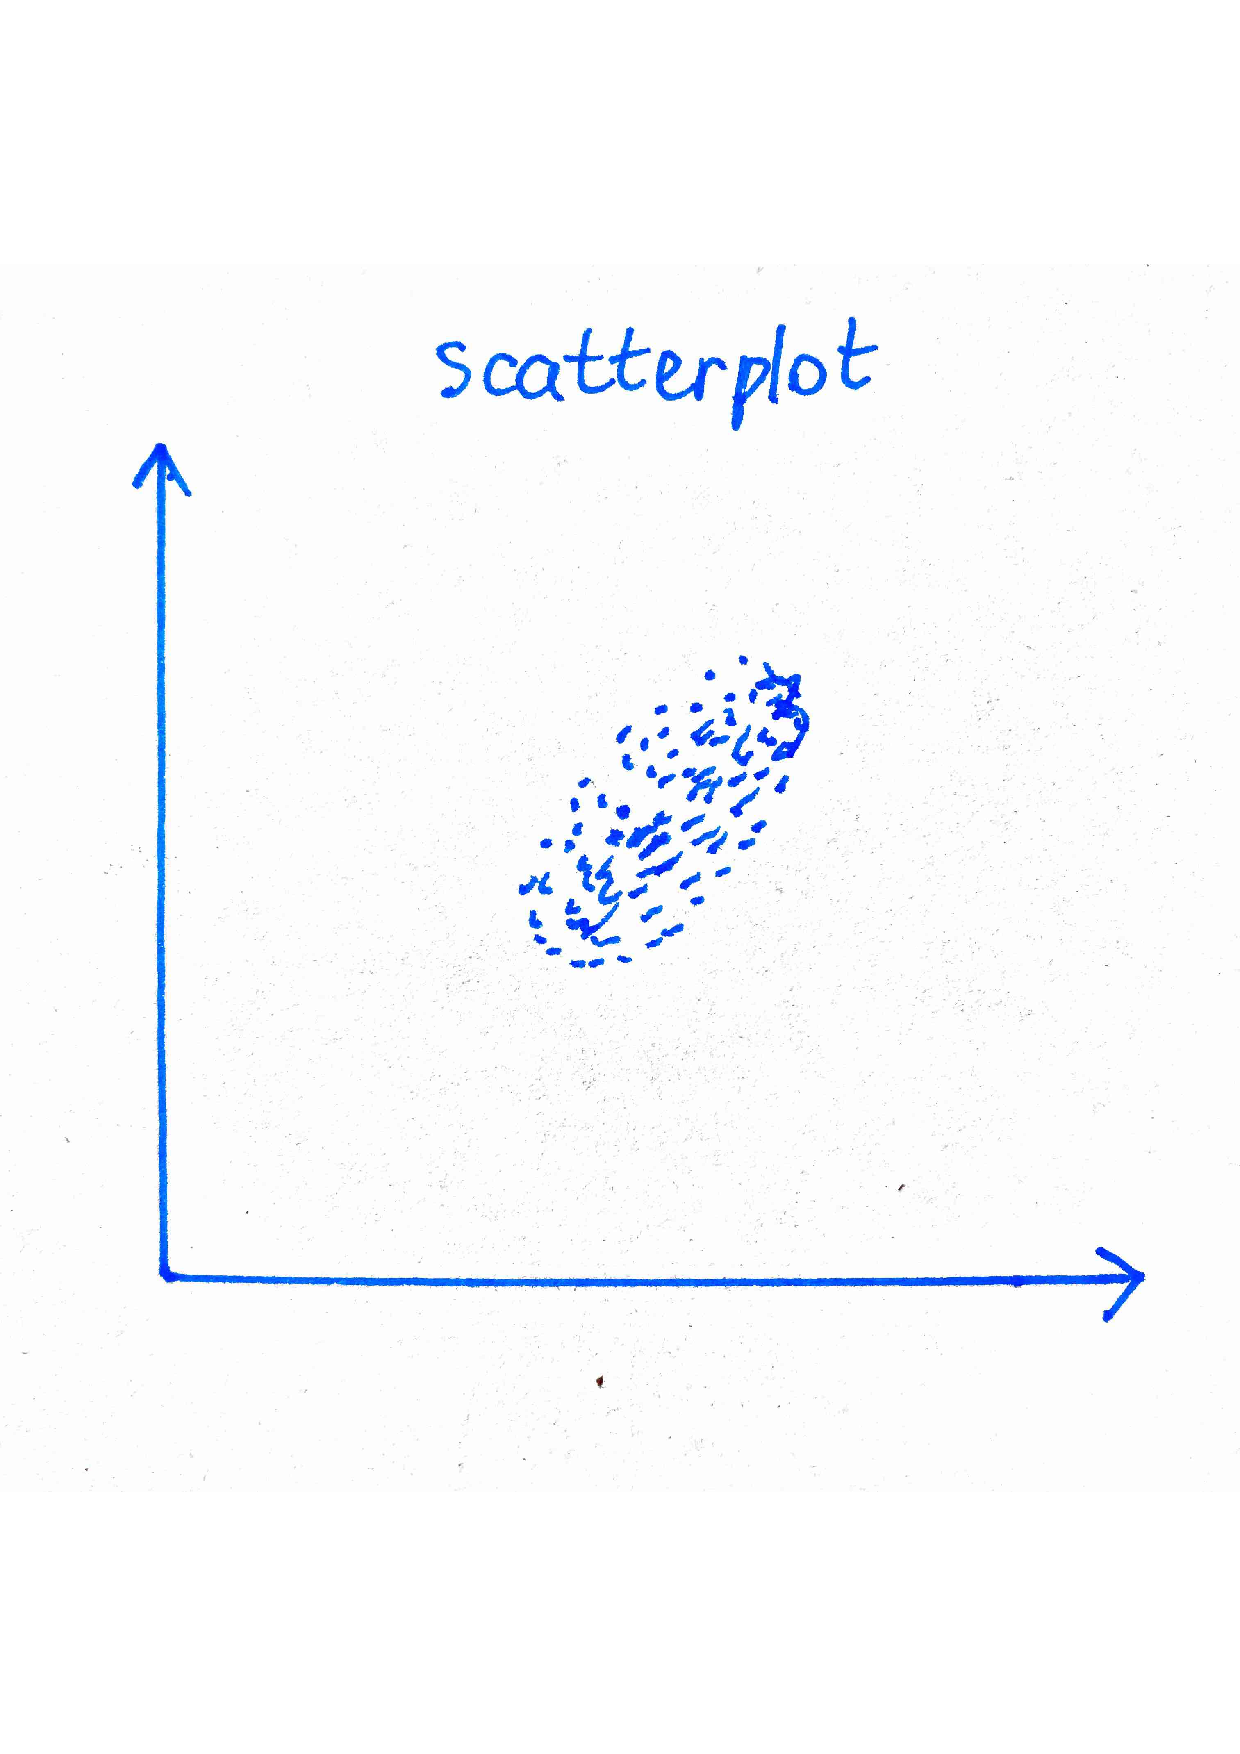
\includegraphics[width=150pt, height=150pt]{p01}
		\captionof{figure}{Данные до стандартизации}
		
	\end{minipage}
	\begin{minipage}{0.51\linewidth}
			\centering
		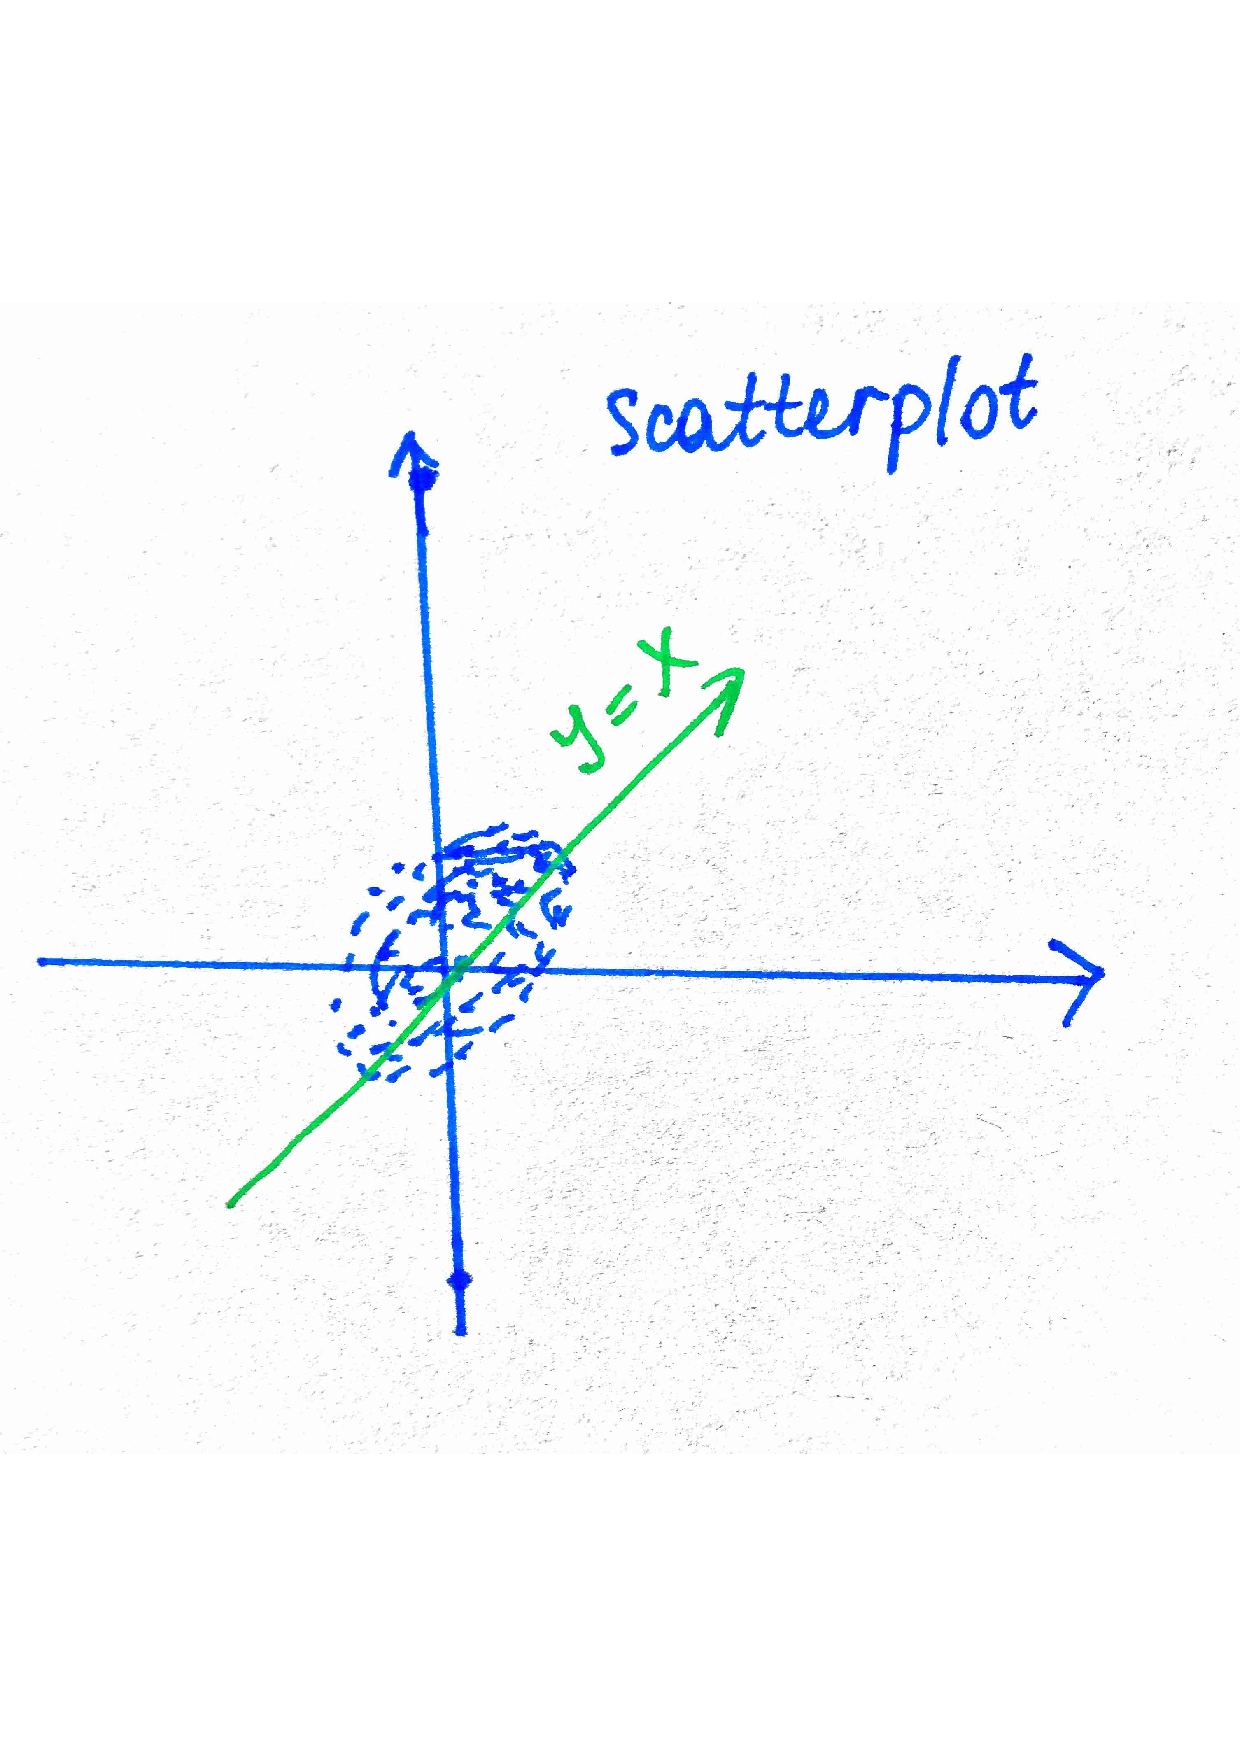
\includegraphics[width=150pt, height=150pt]{p02}
		\captionof{figure}{Данные после стандартизации}
		\label{p02}
	\end{minipage}

\newpage
	\item \textit{Данные с нулевой корреляцией:}
	
	\begin{minipage}{0.51\linewidth}
			\centering
		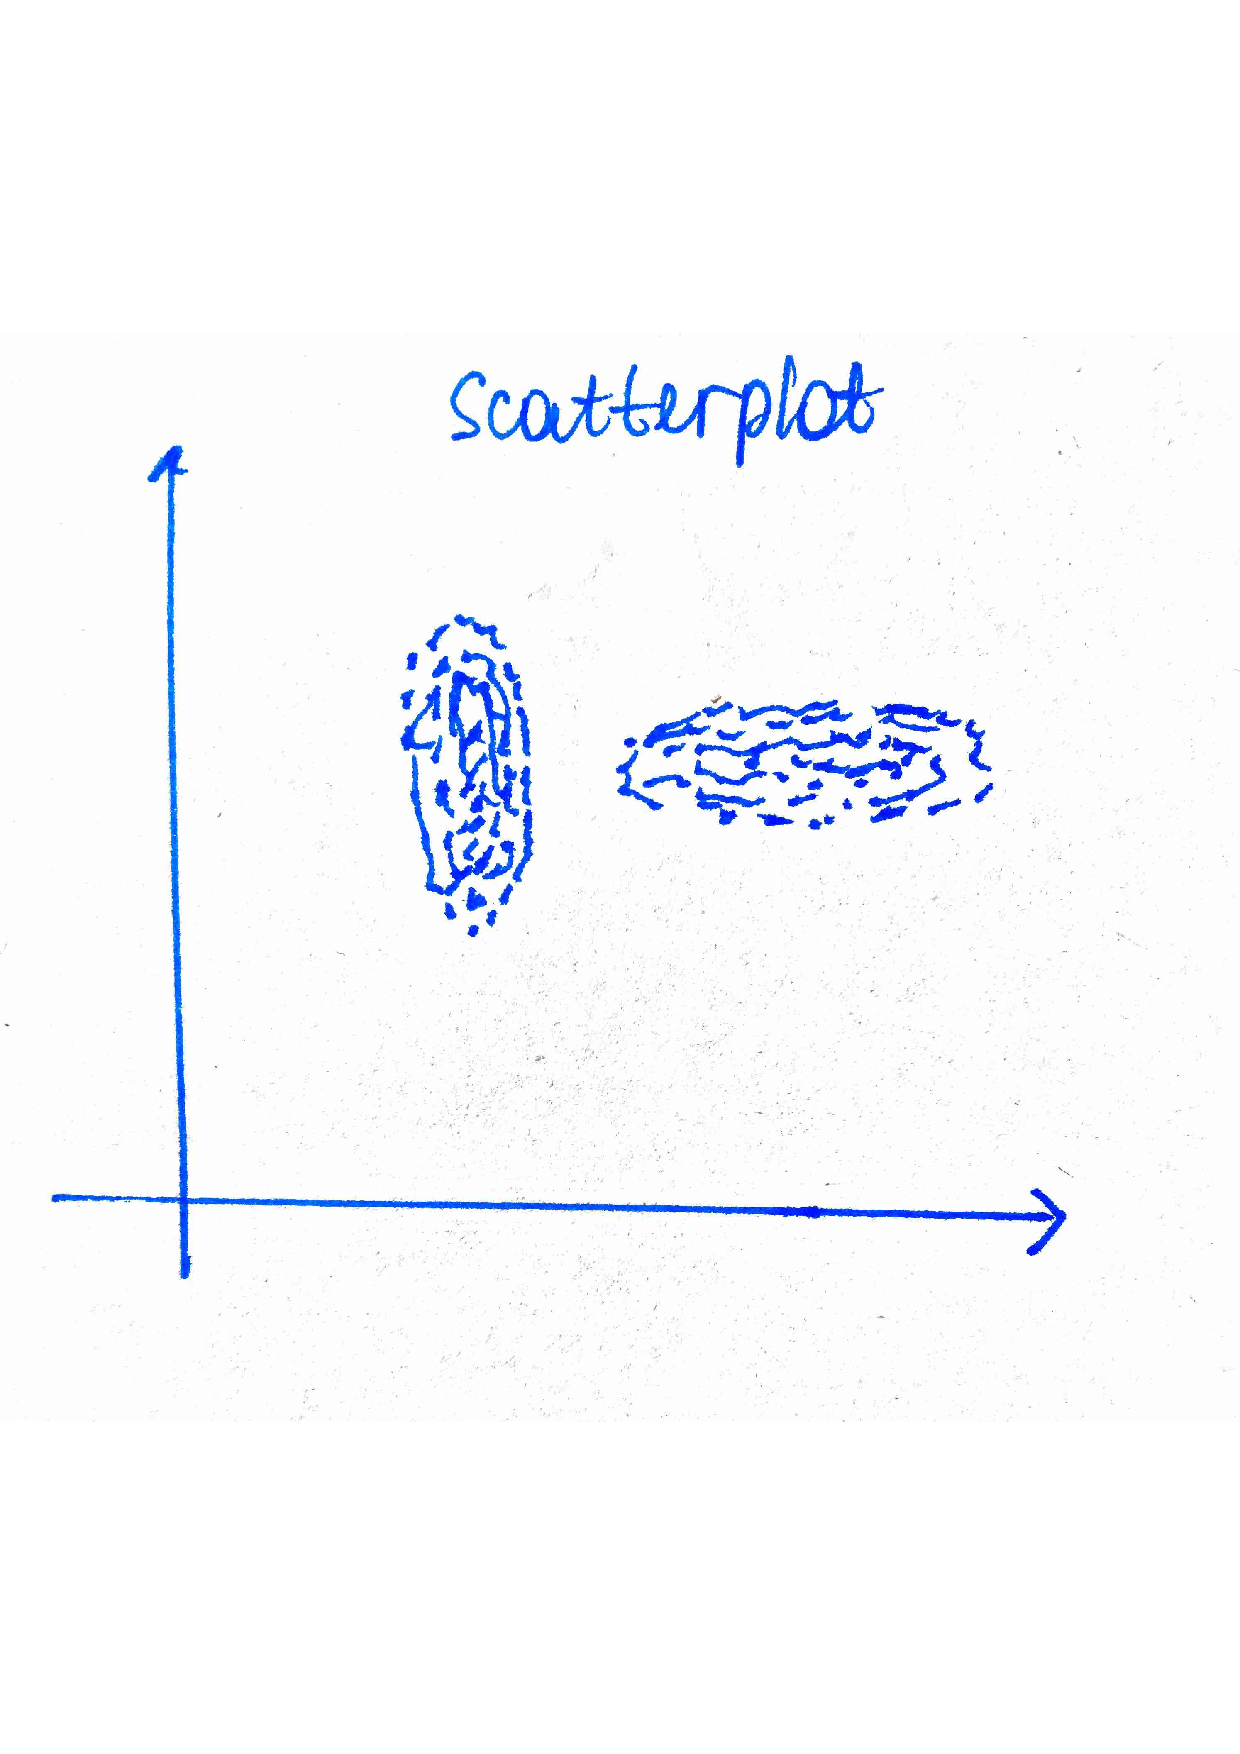
\includegraphics[width=150pt, height=150pt]{p03}
		\captionof{figure}{Данные до стандартизации}
	\end{minipage}
	\begin{minipage}{0.51\linewidth}
			\centering
		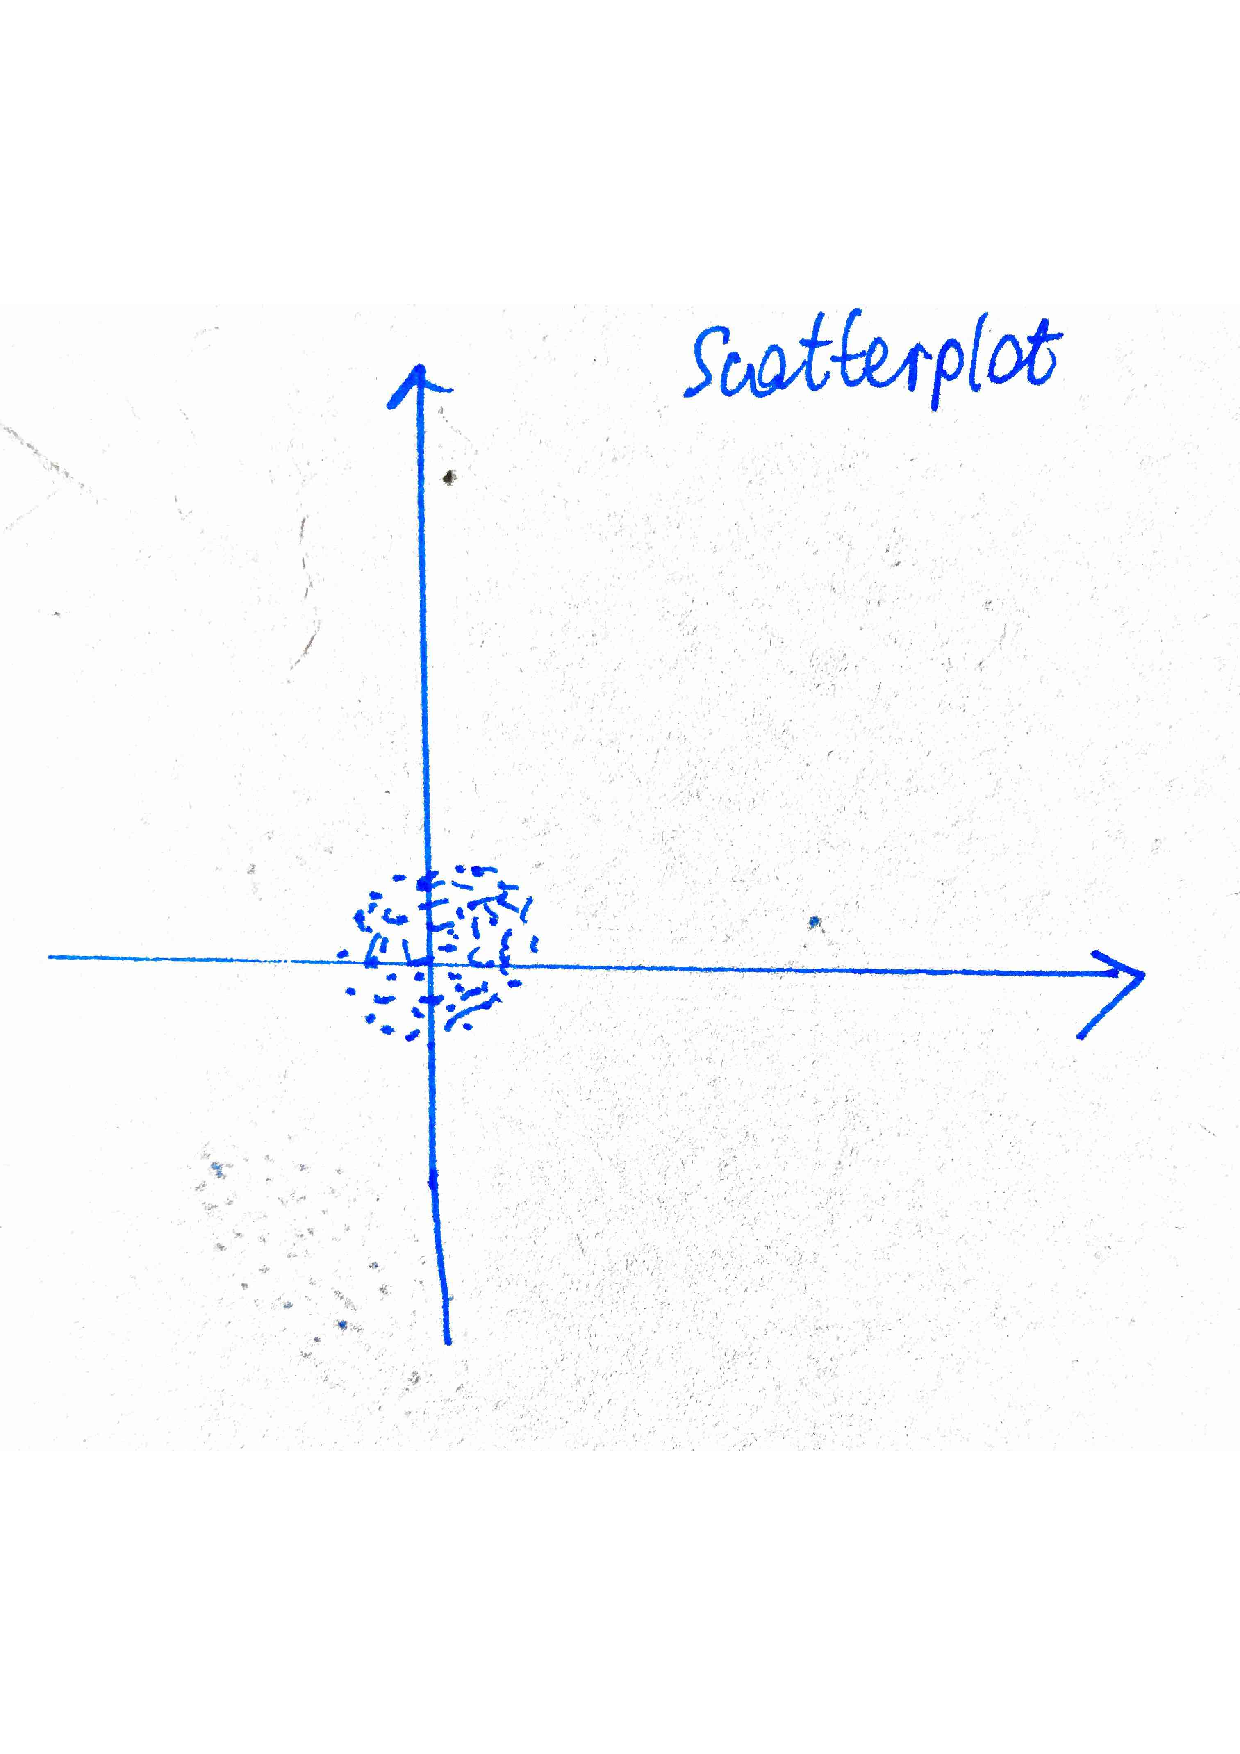
\includegraphics[width=150pt, height=150pt]{p04}
		\captionof{figure}{Данные после стандартизации}
	\end{minipage}
После стандартизации --- круг.
\end{enumerate}

\section{Многомерное нормальное распределение}\label{q1}
Рассмотрим $\bm\xi \sim \mathrm{N}_p(\bm\mu,\bm\Sigma)$, где $\bm\mu = \textsf{E} \bm\xi$ --- вектор из средних значений $\bm\xi$, $\bm\Sigma = \mathrm{Cov} \bm\xi$ --- ковариационная матрица. Предположим, что $\bm\Sigma$ --- невырожденная матрица.\footnote{$|\bm\Sigma| \neq 0$.} \textit{Плотность многомерного нормального распределения} задаётся формулой:
\begin{gather*}
\mathrm{p}(\mathbf{x}, \bm\mu, \bm\Sigma) = \frac{1}{(2\pi)^{p/2} |\bm\Sigma|^{1/2}} \exp \{-\frac{1}{2} (\mathbf{x} - \bm\mu)^{\mathrm{T}}\bm\Sigma^{-1}(\mathbf{x} - \bm\mu)\} \text{ для } \forall \mathbf{x}  \in\mathbb{R}^{p}, \text{ где}
\end{gather*}
$p$ --- количество признаков. Очевидно, что в одномерном случае плотность будет иметь следующий вид:
\begin{gather*}
p(x) = \frac{1}{\sqrt{2 \pi} \sigma} \exp \{-\frac{(x - \mu)^2}{2\sigma^2}\}, \text{ где}
\end{gather*}
$\mu$, $\sigma$ --- числа.
Введём следующее понятие --- \textit{расстояние Махаланобиса}:
\begin{gather*}
r^2_M(\mathbf{x}, \bm\mu, \bm\Sigma) = (\mathbf{x} - \bm\mu)^{\mathrm{T}} \bm\Sigma^{-1} (\mathbf{x} - \bm\mu).
\end{gather*}
Отметим, что $\bm\Sigma$ в данном случае является неотрицательно определённой симметричной матрицей. Но так как ковариационная матрица удовлетворяет данному условию, то получаем, что если расстояния Махаланобиса совпадают, то и плотности многомерного нормального распределения тоже. Посмотрим, что будет являться расстоянием Махаланобиса в одномерном случае ($p = 1$):
\begin{gather*}
\sqrt{\frac{(x - \mu)^2}{\sigma^2}} = \frac{|x - \mu|}{\sigma}=r_M(x,\mu,\sigma^2) \text{ --- \textit{расстояние до мат.ож., измеренное в $\sigma$}}.
\end{gather*}
\textbf{На выборочном языке:} $$\frac{|x_i - \overline{x}|}{s_i}.$$
Таким образом, если у нас есть нормальное распределение, то в одномерном случае мы можем измерять расстояние в сигмах, а в случае многомерного нормального распределения мы смотрим на линии уровня (точки, находящиеся на одном расстоянии Махаланобиса от центра).
\begin{center}
	\begin{minipage}{0.51\linewidth}
		\centering
		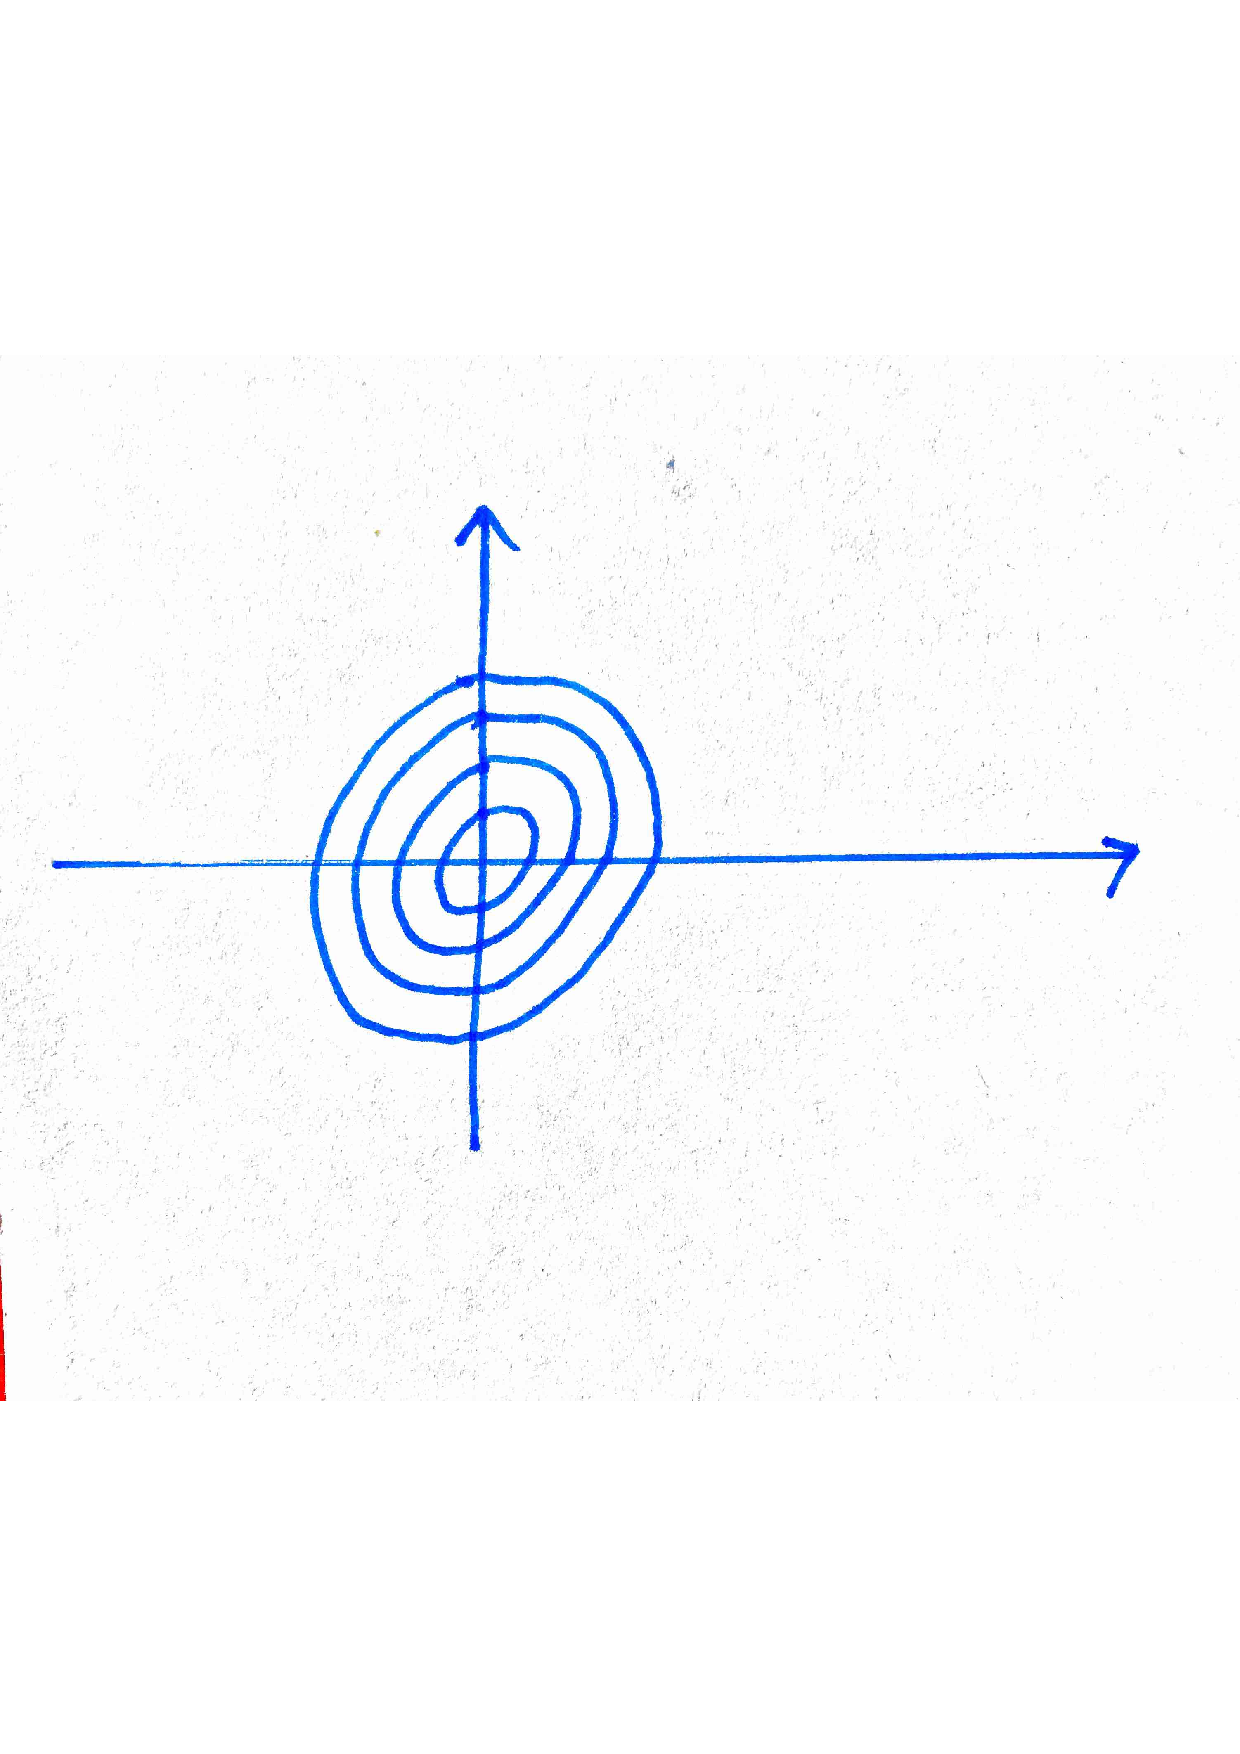
\includegraphics[width=150pt, height=150pt]{p05}
		\captionof{figure}{Линии уровня}
	\end{minipage}
\end{center}


Ответим на следующий вопрос: \textit{какое преобразование необходимо сделать со случайной величиной, имеющей нормальное распределение, чтобы из зависимости получить независимость?}
\begin{center}
	\begin{minipage}{0.8\linewidth}
		\centering
		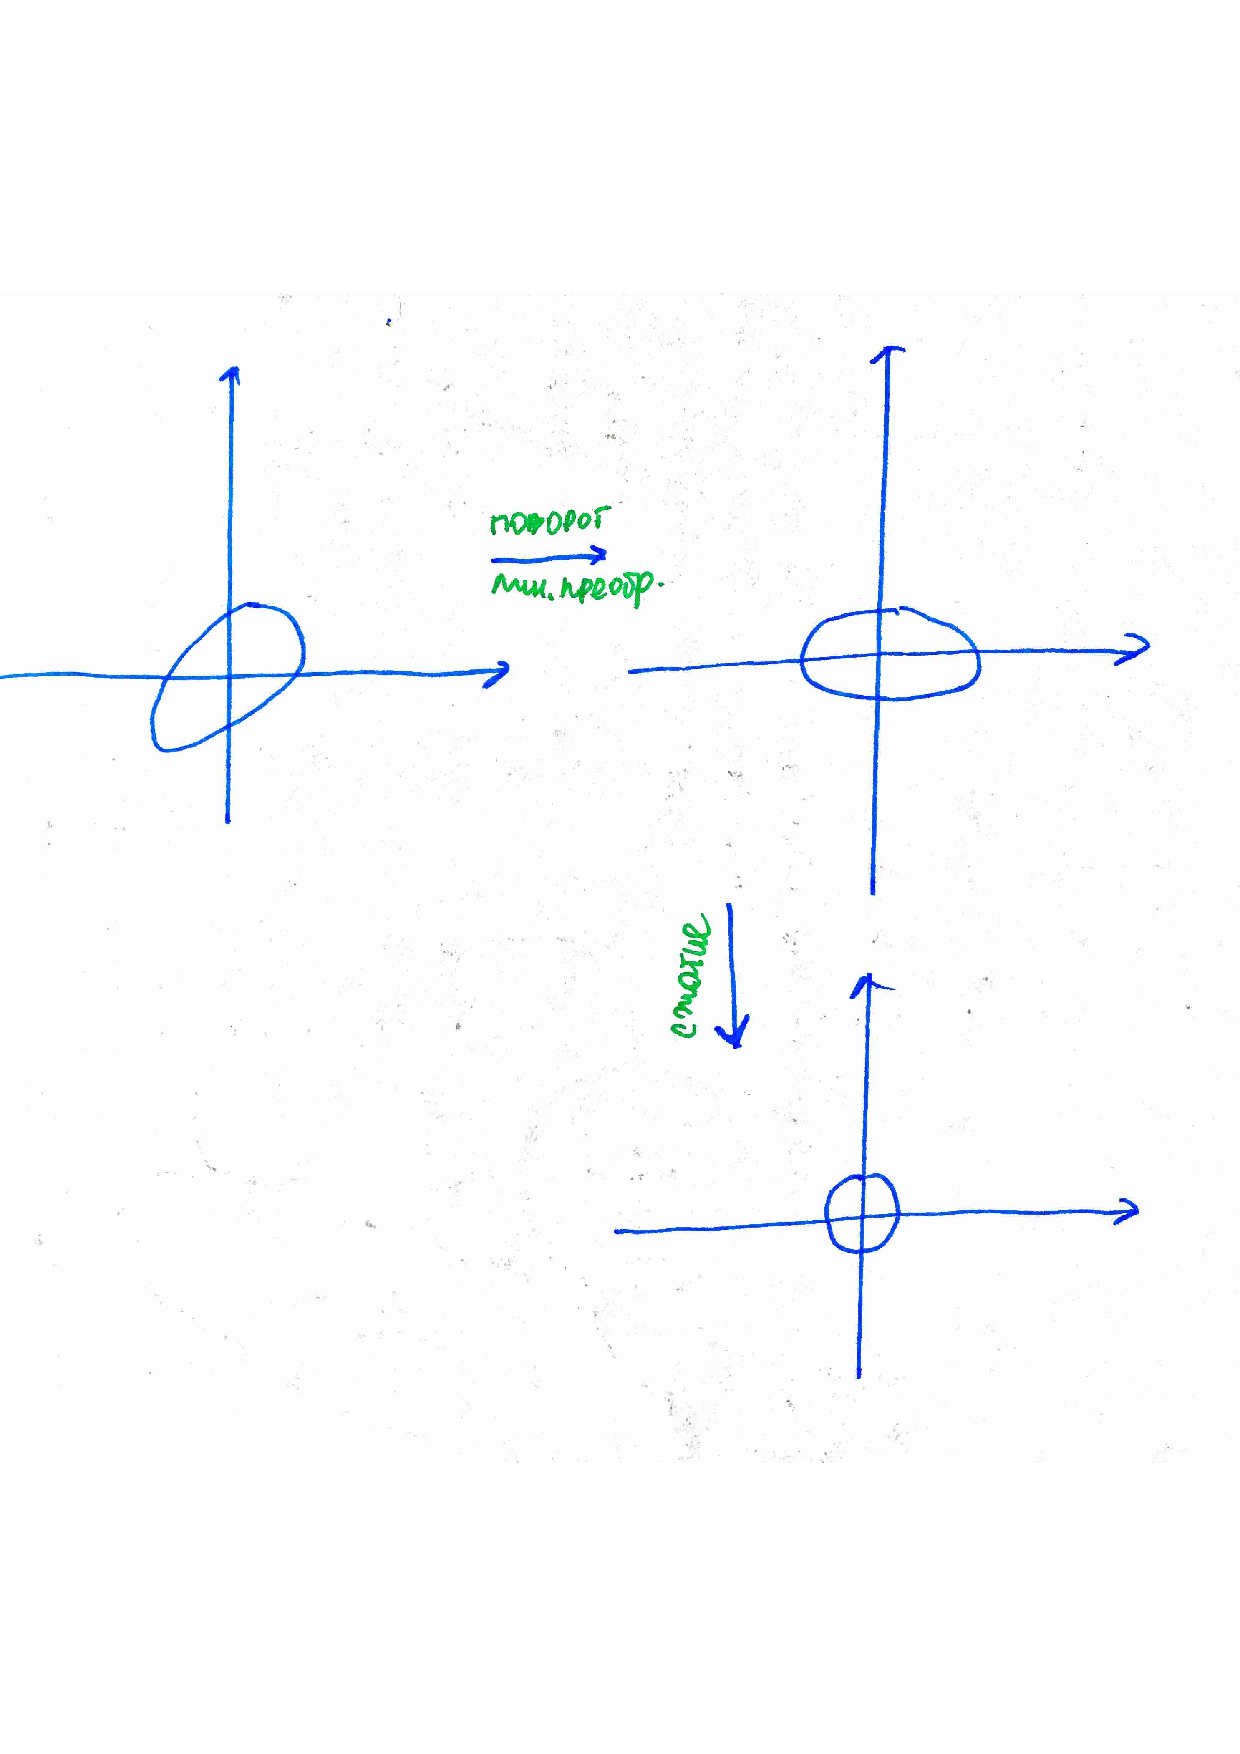
\includegraphics[width=150pt, height=150pt]{p06}
		\captionof{figure}{Отбеливание}
	\end{minipage}
\end{center}

Сначала делаем поворот, а затем стандартизуем. Такое преобразование еще называется ``отбеливанием''.

Пусть $\bm\zeta = \bm\Sigma^{-1/2} (\bm\xi - \bm\mu)$ --- новая случайная величина, полученная из исходной линейным преобразованием. несложно сосчитать, что $\textsf{E}\bm\zeta = \mathbb{O}$, так как $$\textsf{E} \bm\zeta = \bm\Sigma^{-1/2} (\textsf{E} \bm\xi - \bm\mu) = \mathbb{O}.$$
Посчитаем ковариацию $\zeta$:
%\footnote{В данном доказательстве воспользовались симметричностью и неотрицательной определённостью ковариационной матрицы $\bm\Sigma$.}
\begin{gather*}
\text{Cov} (\bm\zeta) = \textsf{E} \bm\zeta \bm\zeta^{\mathrm{T}} =\bm\Sigma^{-1/2} \text{Cov} (\bm\xi) \bm\Sigma^{-1/2} = \bm\Sigma^{-1/2} \underbrace{\bm\Sigma^1}_{\textsf{E}\bm\xi \bm\xi^{\mathrm{T}}} \bm\Sigma^{-1/2} = \mathbb{I}.
\end{gather*}


Вспомним несколько свойств, которые характерны для нормально распределённых случайных величин:
\begin{enumerate}
	\item Если $\xi \sim \mathrm{N}$, то и всякое линейное преобразование $\xi$ тоже имеет нормальное распределение.
	\item Знаем, что из независимости следует некоррелированность. В случае нормального распределения верно и обратное.
	В общем случае это неверно. Приведём пример, когда зависимость есть, но корреляция равна 0.
	\begin{center}
		\begin{minipage}{0.51\linewidth}
			\centering
			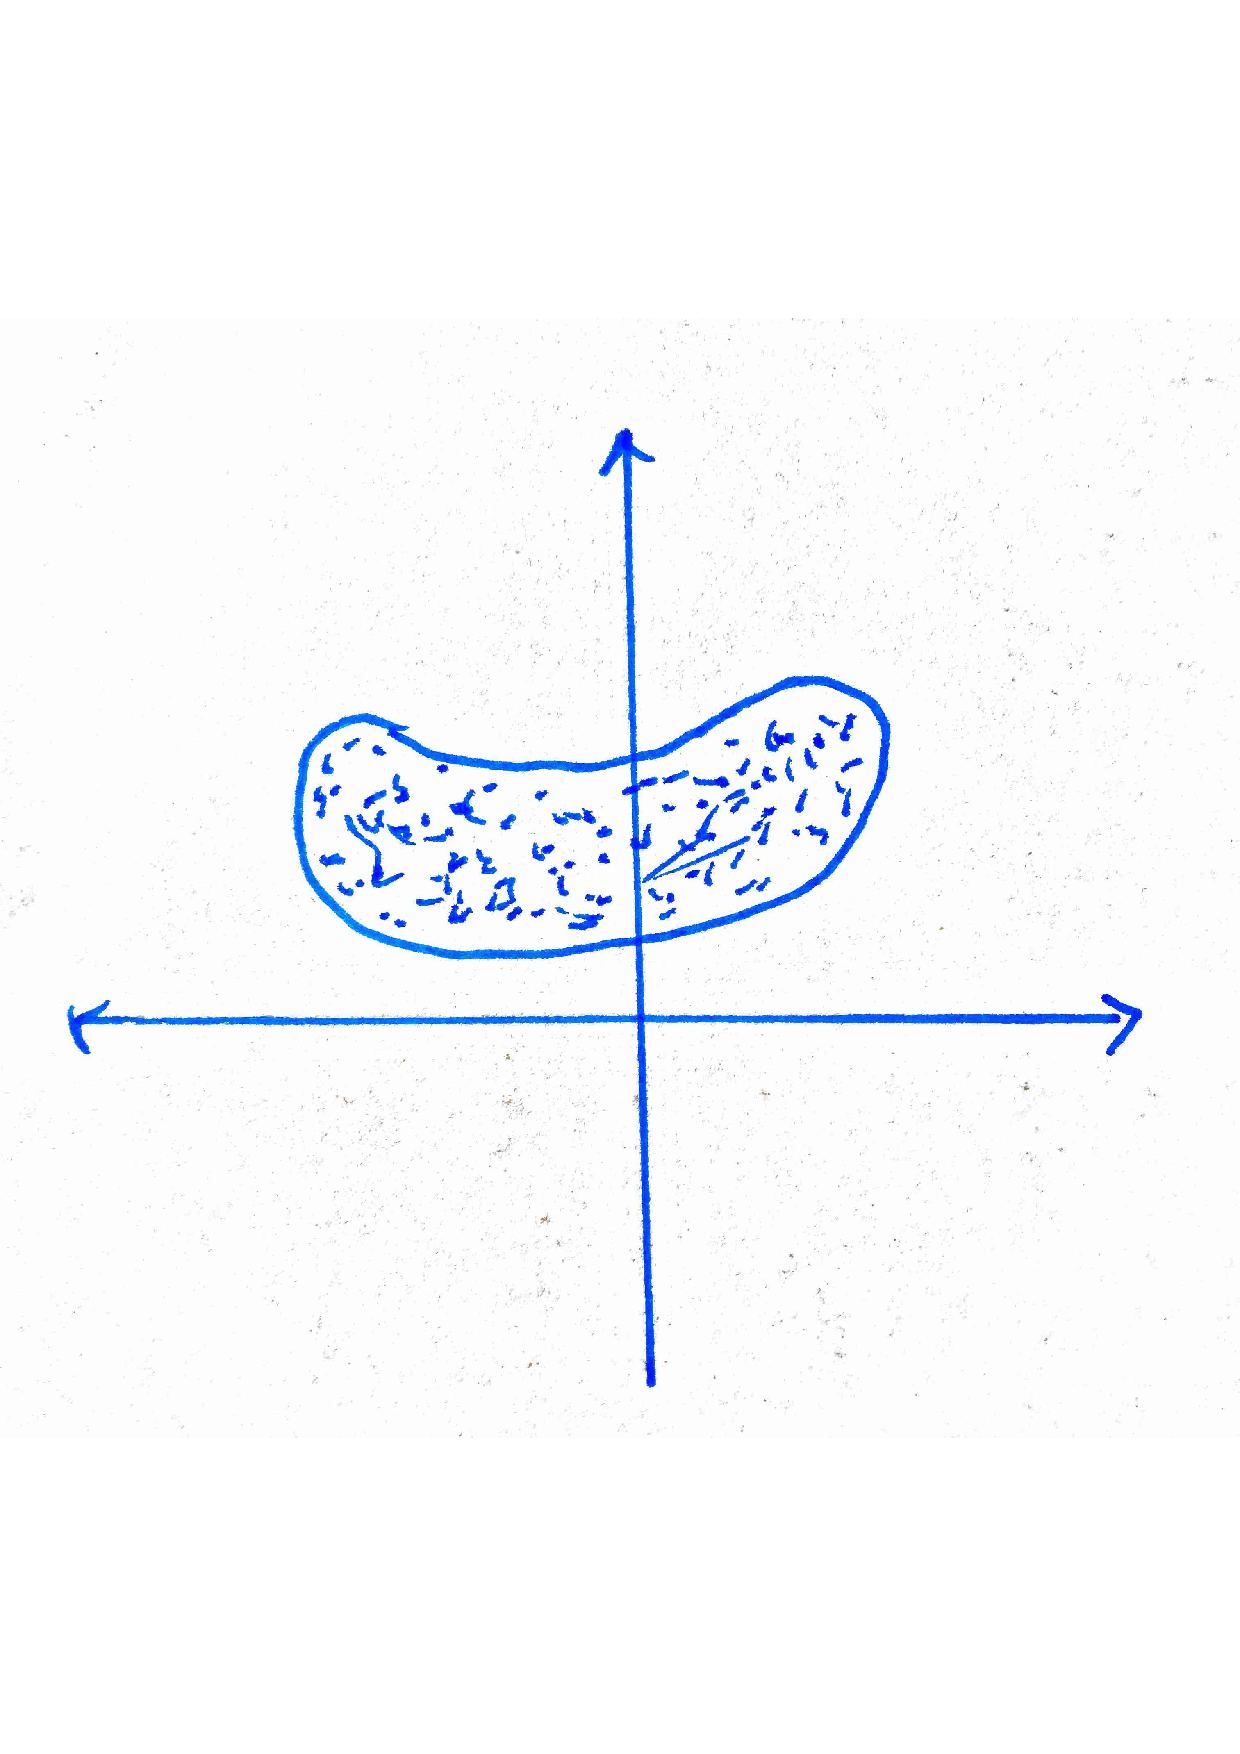
\includegraphics[width=150pt, height=150pt]{p07}
			\captionof{figure}{Пример данных, когда зависимость есть, но корреляция нулевая}
		\end{minipage}
	\end{center}
	\item Условное математическое ожидание является линейной функцией.
	\item Ковариационная матрица $\bm\Sigma$ может быть вырожденной:\footnote{Например, когда двумерное распределение сосредоточено на одной прямой.}
	\begin{center}
		\begin{minipage}{0.4\linewidth}
			\centering
			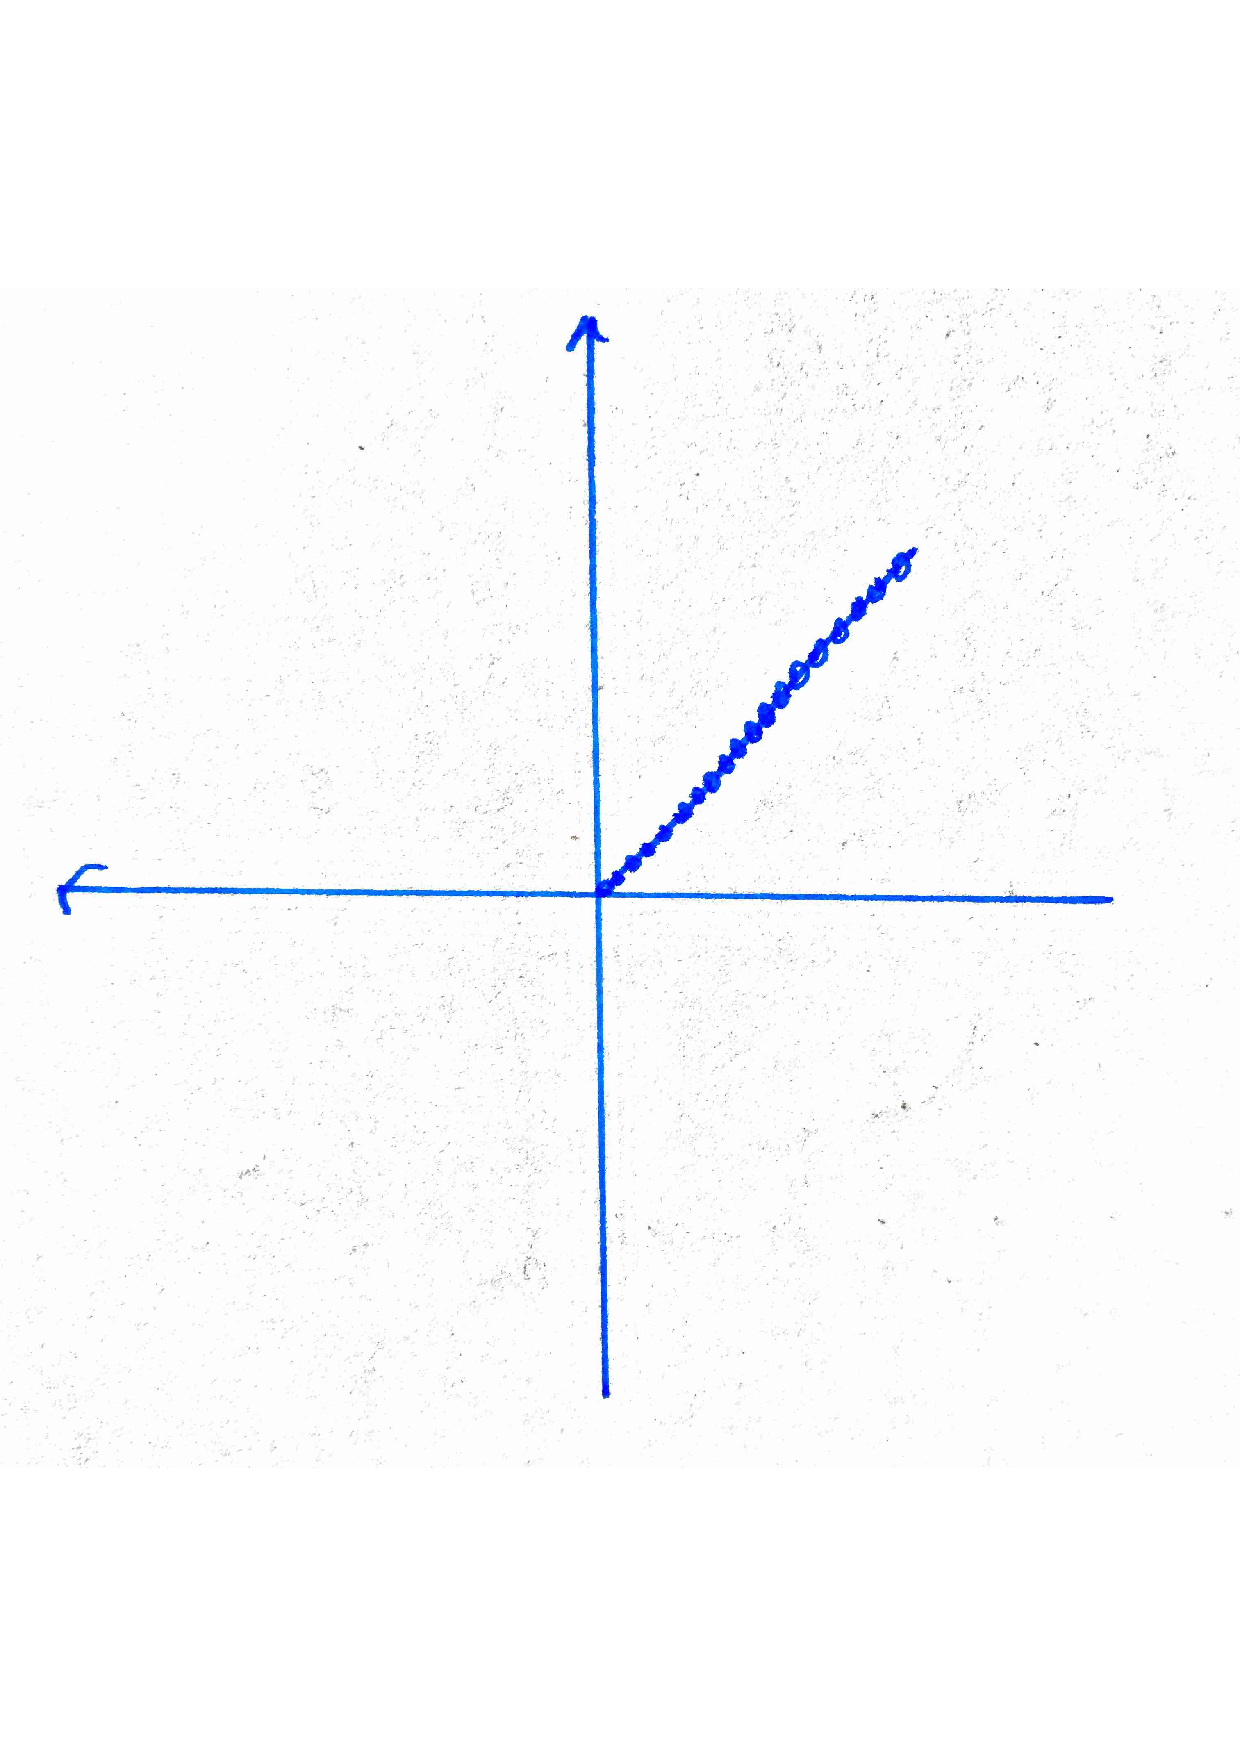
\includegraphics[width=150pt, height=150pt]{p08}
			\captionof{figure}{Ковариационная матрица вырождена}
		\end{minipage}
	\end{center}
	
\end{enumerate}

\section{Переход к новым признакам}
Пусть $\xi$ --- $p$-мерная случайная величина, $p$ --- количество признаков. Считаем, что среднее равно нулю. Хотим образовать новый признак, который является линейной комбинацией старых признаков (смысл в том, чтобы сделать так, чтобы новый признак был в некотором смысле лучше, чем старые):
\begin{gather*}
\eta = \mathbf{A}^{\mathrm{T}}\xi = \xi^{\mathrm{T}} \mathbf{A} = a_1 \xi_1 + \ldots + a_p \xi_p, \hspace{0.3 cm} \mathbf{A} \in \mathbb{R}^p,\\
\textsf{D}\eta = \mathbf{A}^{\mathrm{T}} \mathbf{\bm\Sigma} \mathbf{A}.
\end{gather*}
Теперь пусть $\eta = (\eta_1, \ldots, \eta_d)^{\mathrm{T}} \in \mathbb{R}^d$ --- $d$-мерная случайная величина, т.е. $d$ --- число новых признаков, которая получается из исходной как $\eta = \mathbb{A}^{\mathrm{T}} \xi$, где $\mathbb{A} \in \mathbb{R}^{p\times d}$. Соответствующая ковариационная матрица будет иметь вид $\mathrm{Cov} (\eta) = \mathbb{A}^{\mathrm{T}} \mathbf{\bm\Sigma} \mathbb{A}$.

\textbf{На выборочном языке:} $Z = \sum\limits_{j = 1}^{p} a_j X_j = \mathbb{X} A \in \mathbb{R}^n$ или $\mathbb{Z} = \mathbb{X} \mathbb{A} \in \mathbb{R}^{n \times d}$, где $\mathbb{X} \in \mathbb{R}^{n \times p}$ --- матрица данных.
\\

\begin{enumerate}
	\item Возьмём в качестве индивидов школьников, а в качестве признаков --- оценки по четырём школьным предметам:
	\begin{itemize}
		\item $X_1$ --- оценка по математике;
		\item $X_2$ --- оценка по физике;
		\item $X_3$ --- оценка по русскому;
		\item $X_4$ --- оценка по литературе.
	\end{itemize}
Сами по себе оценки мало несут информации про общее положение в школе или классе, поэтому давайте создадим новые признаки, которые будут более информативными. Пусть это будут
\begin{itemize}
	\item $Z_1 = X_1 + X_2 + X_3 + X_4$ --- сумма оценок по всем предметам;
	\item $Z_2 = X_1 + X_2 - (X_3 + X_4)$ --- разность между оценками по естественным и гуманитарным наукам.
\end{itemize}
Выясним, как будет выглядеть матрица $\mathbb{A}$ в этом случае:
\begin{gather*}
\mathbb{A} = \begin{pmatrix}
1 & 1\\
1 & 1\\
1 & -1\\
1 & -1
\end{pmatrix} \in \mathbb{R}^{4 \times 2}.
\end{gather*}

\item Рассмотрим два признака: оценки по математике $X_1$ и физике $X_2$.

	\begin{center}
	\begin{minipage}{0.51\linewidth}
		\centering
		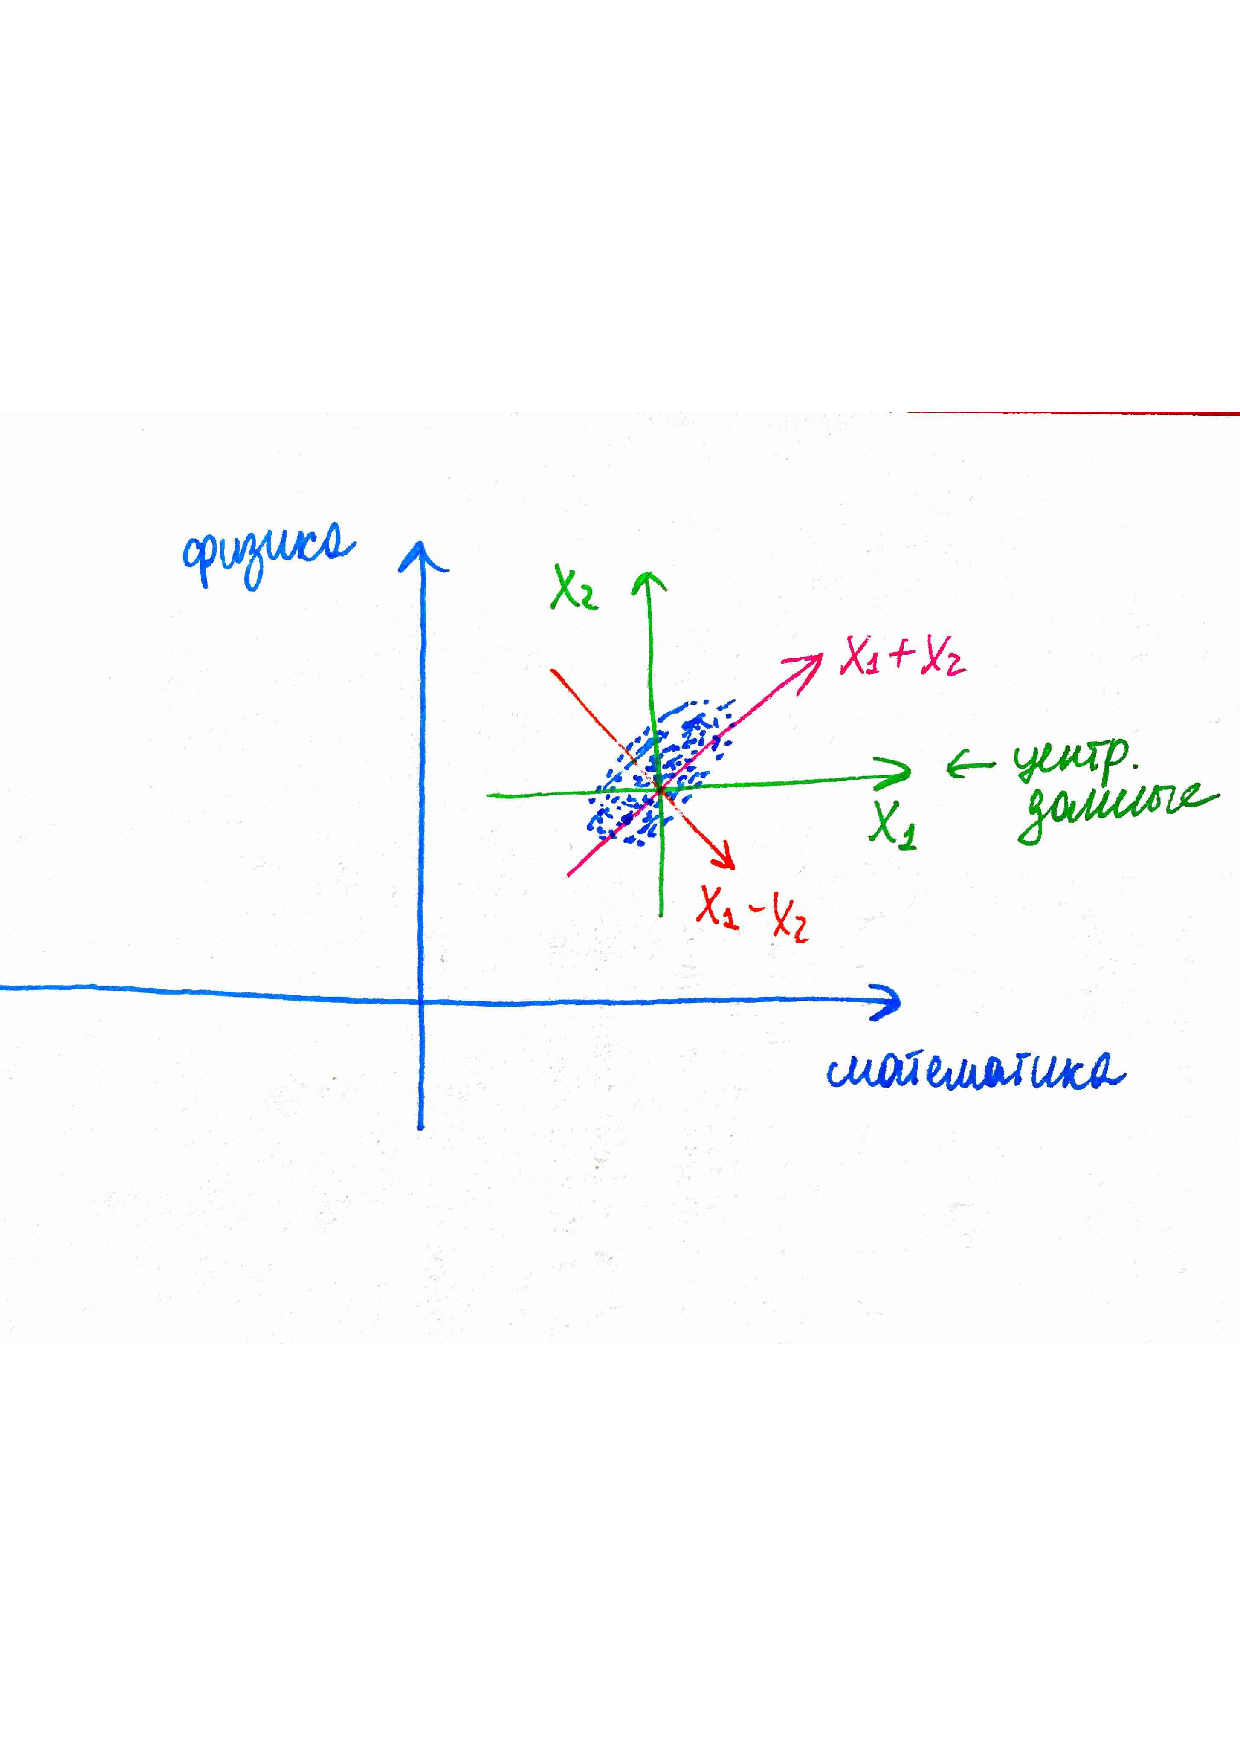
\includegraphics[width=150pt, height=170pt]{p10}
		\captionof{figure}{Scatterplot: $X_1$ and $X_2$}
		\label{10}
	\end{minipage}
\end{center}

В данной ситуации получается, что новый признак $X_1 + X_2$ лучше всего характеризует данные, то есть это та характеристика, по которой ученики максимально различаются; второй признак --- $X_1 - X_2$, по нему ученики отличаются меньше. В анализе главных компонент (АГК) необходимо выбрать признак, который бы наилучшим образом характеризовал данные. Такой характеристикой будет тот признак, по которому данные максимально различаются.

\item  Рассмотрим два признака: оценки по математике $X_1$ и литературе $X_4$. Максимальное отличие получаем по разности данных признаков.\footnote{Нарисуйте scatterplot в этом случае}	

\item Возможно, что данные неоднородные. Тогда новый признак строится так, чтобы по нему группы
максимально различались. Например, если взять математиков и филологов, то данные образуют две группы.

\begin{center}
	\begin{minipage}{0.51\linewidth}
		\centering
		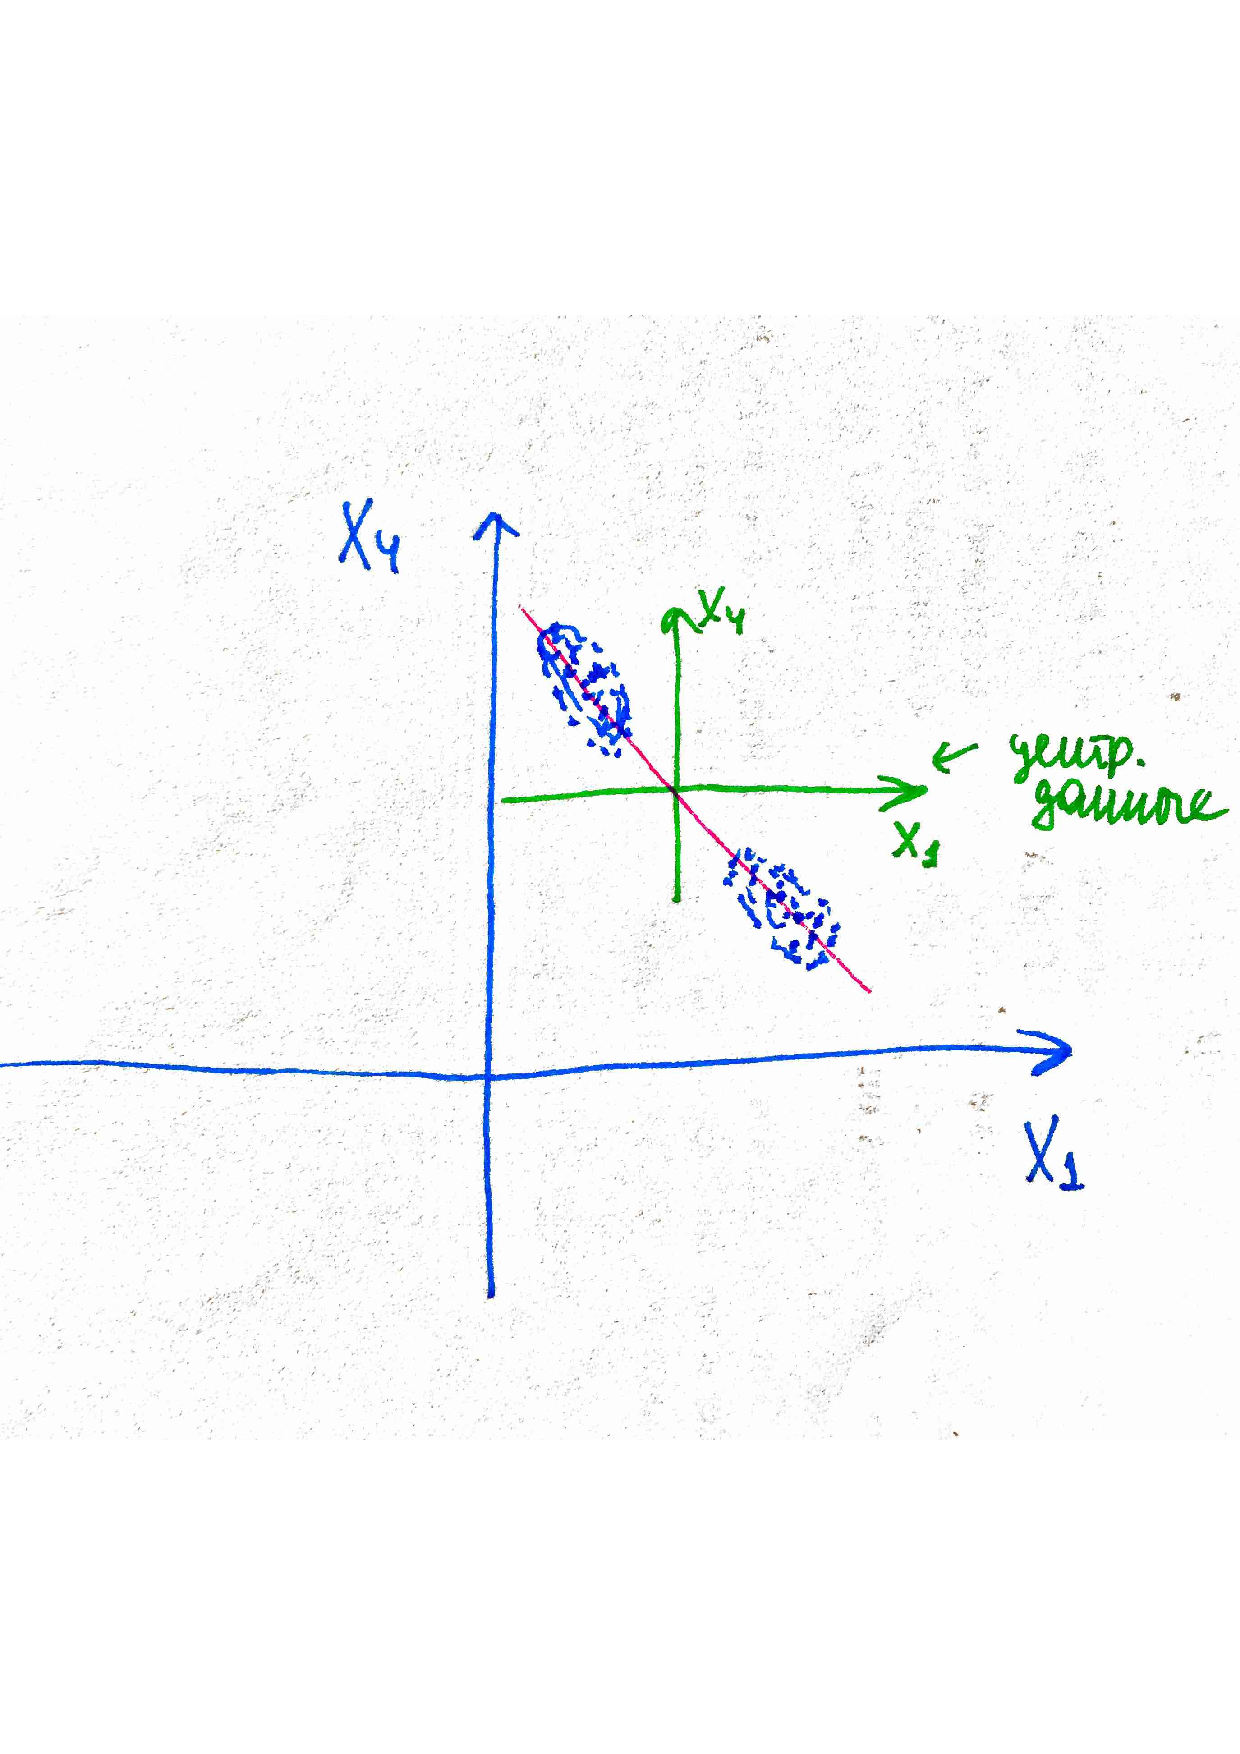
\includegraphics[width=150pt, height=170pt]{p11}
		\captionof{figure}{Scatterplot: $X_1$ and $X_4$}
		\label{10}
	\end{minipage}
\end{center}
\end{enumerate}

\subsection{Две интерпретации новых признаков. Факторные нагрузки}
Обсудили, зачем необходимы новые признаки. Также до этого мы требовали, чтобы новые признаки были линейной комбинацией старых. Теперь добавим еще условие, что:
\begin{itemize}
	\item на выборочном языке: $Z_i \perp Z_j$ (вектора-признаки ортогональны).
	\item на генеральном языке: $\rho(\eta_i, \eta_j) = 0$ (случайные величины-признаки некоррелированы).
\end{itemize}
Зависимость признаков по смыслу означает, что часть одного признака входит в другой, то есть получается некоторая избыточность. Поэтому и требуется независимость (в данном случае, более слабое условие --- некоррелированность).

Пусть $\rnk(\mathbb{X}) = d$, $(Z_1, \ldots, Z_d)$ --- ортогональный базис в подпространстве размерности $d$ --- $\spn(X_1, \ldots, X_p) = \mathrm{colspan}(\mathbb{X})$.
Превратим базис в \textit{ортонормированный базис}: $Q_i = \frac{Z_i}{\Arrowvert Z_i\Arrowvert}$. В ортонормированном базисе удобно вычислять координаты вектора через скалярные произведения с базисными векторами.
Если $U_1, \ldots, U_d$ --- ортономированный базис в $\mathbb{R}^d$, то $\forall$ $A \in \mathbb{R}^d$ раскладывается по ортонормированному базису:
\begin{gather*}
A = \sum\limits_{i = 1}^d <A, U_i> U_i, \text{ где $<A, U_i>$ --- $i$-ая координата вектора $A$ в базисе $\{U_j\}_{j = 1}^d$.}
\end{gather*}
 \footnote{Рассмотрим пример: пространство $\mathbb{R}^2$, соответствующий базис $(1,1)^{\mathrm{T}}/\sqrt{2}$, $(1,-1)^{\mathrm{T}}/\sqrt{2}$. Это ортонормированный базис, да? Как вычислить координаты вектора $(5, 4)^{\mathrm{T}}$ в данном базисе?
}
 Таким образом, $\{Q_i\}_{i=1}^d$ --- ортонормированный базис в пространстве $\spn(X_1, \ldots, X_p)$.


\textit{Новые признаки на самом деле интерпретируются двумя способами:}
\begin{itemize}
	\item Новые признаки задаются равенством (новые признаки есть линейная комбинация старых):
	\begin{gather*}
	\mathbb{X}\mathbb{A} = \mathbb{Z}.
	\end{gather*}
	\item Исходные признаки выражаются через новые (есть пространство, в нём базис, каждый вектор этого пространства раскладывается по базису):
	\begin{gather}\label{1}
	\forall \hspace{0.1 cm} i = 1,\ldots,p \hspace{0.4 cm} X_i = \sum\limits_{j = 1}^d <X_i, Q_j> Q_j.
	\end{gather}
\end{itemize}
\begin{definition}
	$f_{ij} = <X_i, Q_j>$ --- факторные веса, факторные нагрузки.
\end{definition}

%\end{document}

Составим матрицу $\mathbb{F} = \{f_{ij}\}_{i = 1, j = 1}^{p,d}= [F_1,:\ldots:F_d] \in \mathbb{R}^{p \times d}$ --- коэффициенты разложения по ортонормированному базису, тогда можем записать разложение \eqref{1} в матричном виде:
\begin{gather}\label{2}
\mathbb{X} = \sum\limits_{j = 1}^d Q_j F_j^{\mathrm{T}} = \mathbb{Q}\mathbb{F}^{\mathrm{T}}.
\end{gather}
$\Arrowvert Q_j\Arrowvert = 1$, $\Arrowvert F_j\Arrowvert \neq 1$ в разложении \eqref{2}. Давайте нормируем $F$. Пусть $\sigma_j = \Arrowvert F_j\Arrowvert$, $P_j = \frac{F_j}{\Arrowvert F_j\Arrowvert}$, тогда $\Arrowvert Q_j\Arrowvert = \Arrowvert P_j\Arrowvert = 1$ и
\begin{gather}\label{3}
\mathbb{X} = \sum\limits_{j = 1}^d \sigma_j Q_j P_j^{\mathrm{T}} = \mathbb{Q} \mathbf{\bm\Sigma} \mathbb{P}^{\mathrm{T}}, \text{ где $\mathbf{\bm\Sigma} = \diag\{\sigma_1, \ldots, \sigma_d\}$.}
\end{gather}
\textit{Что за матрица $Q_jP_j^{\mathrm{T}} \in \mathbb{R}^{n \times p}$?} Можно заметить, что $\rnk(Q_jP_j^{\mathrm{T}}) = 1$; действительно, столбцы матрицы пропорциональны; то же самое для строк. Таким образом, у нас была исходная матрица ранга $d$, а мы превратили её в сумму $d$ элементарных матриц ранга 1.

%\begin{proposition}
%	$\mathbf{\bm\Sigma}\mathbb{P}^{\mathrm{T}} = \mathbb{F}^{\mathrm{T}}$.
%\end{proposition}
%\begin{proof}[Доказательство.]
%	\textcolor{red}{И это бы надо бы пояснить}
%\end{proof}

Пусть $\mathbb{X}^{(j)} = \sigma_jQ_jP_j^{\mathrm{T}}$, тогда $\mathbb{X} = \sum\limits_{j = 1}^d \mathbb{X}^{(j)}$.
\subsection{Вклад новых признаков}
Ввели новый признак, теперь хотелось бы понять, какую важную часть информации он в себя включает. Введём скалярное произведение двух матриц, которой соответствует норма Фробениуса ($\Arrowvert \mathbb{A}\Arrowvert^2_F = \sum\limits_{ij}a_{ij}^2$):
\begin{gather*}
(\mathbb{Y}, \mathbb{Z})_F = \sum\limits_{i, j} y_{ij} z_{ij}.
\end{gather*}

Если верно $\Arrowvert\mathbb{X}\Arrowvert^2 = \Arrowvert\sum\limits_{j = 1}^d \mathbb{X}^{(j)}\Arrowvert^2_F \stackrel{?}{=} \sum\limits_{j = 1}^d\Arrowvert\mathbb{X}^{(j)}\Arrowvert^2_F$, то \textit{вклад $j$-ого признака} (вклад $j$-ой элементарной матрицы) равен $\frac{\Arrowvert\mathbb{X}^{(j)}\Arrowvert^2}{\Arrowvert\mathbb{X}\Arrowvert^2}$.\footnote{Если отношение равно $1/2$, то значит, что $j$-ый признак измеряет $50\%$ всей информации.}
\begin{remark}
	Для разложения \eqref{3}, $\Arrowvert\sum\limits_{j = 1}^d \mathbb{X}^{(j)}\Arrowvert^2_F = \sum\limits_{j = 1}^d\Arrowvert\mathbb{X}^{(j)}\Arrowvert^2_F$ (скалярное произведение равно 0, потому что $Q_i \perp Q_j$).
\end{remark}

Так как $Q_j$ и $P_j$ нормированы, то можем продолжить равенство:
\begin{gather*}
\Arrowvert\mathbb{X}\Arrowvert^2 = \Arrowvert\sum\limits_{j = 1}^d \mathbb{X}^{(j)}\Arrowvert^2_F = \sum\limits_{j = 1}^d\Arrowvert\mathbb{X}^{(j)}\Arrowvert^2_F = \sum\limits_{j = 1}^d \sigma_j^2.
\end{gather*}

\begin{remark}
	Пусть старые признаки $X_i$ центрированные, тогда новые признаки $Z_i$ и $Q_i$ тоже центрированные.
\end{remark}
\begin{proof}[Доказательство.]
	 Новые признаки --- это линейная комбинация старых. Среднее линейной комбинации есть линейная комбинация средних по признакам. Средние по признакам равны 0, получаем центрированные новые признаки.
\end{proof}

\section{Пара фактов из линейной алгебры}
\begin{enumerate}
	\item \textit{Унитарная матрица} $\mathbb{U}$ --- ортогональная матрица в комплексном случае. Ее свойства:
	\begin{itemize}
		\item $\mathbb{U}$ --- квадратная матрица: $\mathbb{U}^{\mathrm{T}} =\mathbb{U}^{-1}$.
		\item Столбцы $\mathbb{U}$ ортонормированы.
		\item Строки $\mathbb{U}$ ортонормированы.\footnote{2 пункт эквивалентен 3. \textit{Почему?} Если матрица ортогональная, то и транспонированная к ней тоже ортогональная (следует из пункта 1).}
\item Умножение на матрицу $\mathbb{U}$ означает \textit{поворот} или \textit{отражение}.
\item При умножении на матрицу $\mathbb{U}$ (и на $\mathbb{U}^\mathrm{T}$) не меняются нормы векторов и углы между векторами. Пусть есть вектора $Y$, $Z$, после умножения на матрицу $\mathbb{U}$ получим $\widetilde{Y} = \mathbb{U}Y,~ \widetilde{Z}=\mathbb{U}Z$ и $\|Y\| = \|\widetilde{Y}\|$, $\|Z\| = \|\widetilde{Z}\|$, $<Y,Z> = <\widetilde{Y}, \widetilde{Z}>$ (почему это означает равенство углов
    между векторами?).
	\end{itemize}


\begin{example}
	 $\mathbb{U} = \begin{pmatrix}
	\cos \phi & \sin \phi\\
	-\sin \phi & \cos \phi
	\end{pmatrix}$ --- матрица поворота на угол $\phi$.
\end{example}

Обычно, унитарная матрица строится из ортонормированного базиса, который составляет столбцы
матрицы. (Проверьте, что в примере с поворотом на $\phi$ это так.)

\item Пусть $\{P_i\}_{i = 1}^r$ --- система независимых векторов, рассмотрим линейную оболочку $\mathcal{L}_r = \spn\{P_1, \ldots, P_r\}$ в $\mathbb{R}^L$, $\Pi: \mathbb{R}^L \rightarrow \mathcal{L}_r$ --- ортогональный проектор на $\mathcal{L}_r$ (он сопоставляет вектору ближайшую точку из подпространства,
    что делается опусканием перпендикуляра). Матрица $\Pi$:
\begin{gather*}
\Pi = \mathbb{P} (\mathbb{P}^{\mathrm{T}} \mathbb{P})^{-1} \mathbb{P}^{\mathrm{T}}.
\end{gather*}
Пусть $\{P_i\}_{i = 1}^r$ --- ортонормированный базис $\mathcal{L}_r$, т.е.
\begin{gather*}
\mathbb{P}^{\mathrm{T}}\mathbb{P} = \mathbb{I}_{r\times r} =  \begin{pmatrix}
1 & \cdots & 0\\
& \ddots & \\
0 & \cdots & 1
\end{pmatrix} \in \mathbb{R}^{r \times r}.
\end{gather*}
Тогда  $\Pi = \mathbb{P} \mathbb{P}^{\mathrm{T}}$.
\end{enumerate}

\newpage
\chapter{Сингулярное разложение\\ (SVD --- Singular Value Decomposition)}
\section{Как строится сингулярное разложение}
Пусть $L$ --- число признаков, $K$ --- количество индивидов, $\mathbb{Y} = \mathbb{X}^{\mathrm{T}} \in \mathbb{R}^{L \times K}$ --- ненулевая матрица. Обозначим $\mathbb{S} = \mathbb{Y}\mathbb{Y}^{\mathrm{T}} \in \mathbb{R}^{L \times L}$ --- симметричная неотрицательно определённая матрица. По определению,
\begin{gather*}
\mathbb{S} U_i = \lambda_i U_i, \text{ где}
\end{gather*}
$\{U_i\}_{i = 1}^L$ --- ортонормированный набор из собственных векторов матрицы $\mathbb{S}$, \\
$\lambda_1 \geq \ldots \geq \lambda_L \geq 0$ --- собственные числа матрицы $\mathbb{S}$.\footnote{Неотрицательные, так как матрица $\mathbb{S}$ неотрицательно определена.}


Пусть $d = \rnk \mathbb{Y} = \mathrm{colrank} \mathbb{Y} = \mathrm{rowrank}\mathbb{Y}$. Знаем, что $d \leq \min (L,K)$.
\begin{proposition}
\begin{enumerate}
	\item $d = \rnk \mathbb{Y} \mathbb{Y}^{\mathrm{T}}$.
	\item $\lambda_d > 0$; $\lambda_i = 0$ при $i > d$.\footnote{Упорядочили собственные числа: первые $d$ строго положительные, а остальные все нули.}
	\item $\{U_i\}_{i = 1}^d$ образуют ортонормированный базис $\mathrm{colspan} \mathbb{Y}$.
\end{enumerate}	
\end{proposition}

Введём вектор
\begin{gather*}
V_i \stackrel{def}{=} \frac{\mathbb{Y}^{\mathrm{T}}U_i}{\sqrt{\lambda_i}} \in \mathbb{R}^k, \hspace{0.2 cm} i = 1, \ldots, d.
\end{gather*}
\begin{proposition}
	\begin{enumerate}
		\item $\{V_i\}_{i = 1}^d$ --- ортонормированная система векторов.
		\item $V_i$ --- собственные вектора $ \mathbb{Y}^{\mathrm{T}}\mathbb{Y}$, соответствующие тем же собственным числам $\lambda_i$. Остальные собственные вектора $ \mathbb{Y}^{\mathrm{T}}\mathbb{Y}$ соответствуют нулевым собственным числам.
		\item $U_i = \displaystyle{\frac{\mathbb{Y}V_i}{\sqrt{\lambda_i}}}$.
		\item $\mathbb{Y} = \sum\limits_{i = 1}^d \sqrt{\lambda_i} U_i V_i^{\mathrm{T}}$ --- SVD (Сингулярное разложение матрицы).\footnote{Разложение в сумму элементарных матриц.}\footnote{Самый важный пункт утверждения.}
	\end{enumerate}
\end{proposition}
\textit{Что здесь считать новыми признаками, если $\mathbb{Y} = \mathbb{X}^{\mathrm{T}}$}? $V_i$,\footnote{Они длинные :)} так как $U_i \in \mathbb{R}^L$, $V_i \in \mathbb{R}^K$.
\begin{itemize}
	\item $U_i$ --- ортонормированный базис в пространстве столбцов.
	\item $V_i$ --- ортонормированный базис в пространстве строк.\footnote{Можем $\mathbb{X}$ транспонировать, проделать всё то же самое, а поменяются местами только $U_i$ и $V_i$.}
	\item $\displaystyle\frac{\lambda_i}{\sum_{i=1}^d \lambda_i}$ --- вклад $i$-ого признака.
\end{itemize}
 \begin{definition}
 		$\sqrt{\lambda_i}$ --- \textit{сингулярные числа} матрицы $\mathbb{Y}$, $U_i$ --- \textit{левые сингулярные вектора}, $V_i$ --- \textit{правые сингулярные вектора}.
 		
 	Тройка $(\sqrt{\lambda_i},U_i,V_i)$ называется $i$-ой собственной тройкой сингулярного разложения.
 \end{definition}

\begin{remark}
	Сингулярное разложение --- единственное разложение с двумя ортонормированными базисами.
\end{remark}

\section{Матричный вид сингулярного разложения}
Можно записать двумя способами:
\begin{enumerate}
	\item Введём $\mathbb{U}_d = [U_1: \ldots: U_d]$, $\mathbb{V}_d = [V_1: \ldots: V_d]$, $\Lambda_d = \diag(\lambda_1, \ldots, \lambda_d)$. Тогда
	\begin{gather*}
	\mathbb{Y} = \mathbb{U}_d\Lambda_d^{1/2}\mathbb{V}_d^{\mathrm{T}}.
	\end{gather*}
	\item Возьмём $\mathbb{U} = [U_1: \ldots: U_d: U_{d+1}: \ldots: U_L]$ --- ортонормированный базис в $\mathbb{R}^L$.\footnote{$U_{d+1}, \ldots, U_L$ соответствуют нулевому собственному числу матрицы.}\\
	$\mathbb{V}^\mathrm{T} = [V_1: \ldots: V_d: V_{d+1}: \ldots: V_K]$ --- ортонормированный базис в $\mathbb{R}^K$.\\
	$\Lambda = \begin{pmatrix}
	\lambda_1 & 0 & \ldots & \ldots & 0\\
	0 & \ddots & & 0 & 0\\
	0 & & \lambda_d & & 0&\\
	0 & & & \ddots & 0\\
	0 & 0 & \ldots & & 0 &
	\end{pmatrix} \in \mathbb{R}^{L \times K}$. Тогда\footnote{$\mathbb{U}, \mathbb{V}$ --- ортогональные матрицы.}
	\begin{gather*}
	\mathbb{Y} = \mathbb{U} \Lambda^{1/2} \mathbb{V}^{\mathrm{T}}.
	\end{gather*}
	~\\
\end{enumerate}

%\end{document}
\section{Единственность сингулярного разложения}
\textit{Насколько единственно разложение SVD (оно одно существует для матрицы или нет)}?
Можно подумать, что разложение не единственное, так как
\begin{enumerate}
	\item Собственные вектора не единственные, то есть если $U_i$ --- собственный вектор, то $(-U_i)$ --- собственный вектор,\footnote{В вещественном случае собственный вектор определяется единственным образом с точностью до константы, модуль которой равен 1 (это всего 1 и -1). Но сингулярное разложение обобщается в комплексном случае, а здесь уже констант, по модулю равных 1, много.}
	\begin{gather*}
	\mathbb{Y} = \sum\limits_{i = 1}^d \sqrt{\lambda_i}U_i V_i^{\mathrm{T}} = \sum\limits_{i = 1}^d \sqrt{\lambda_i}(-U_i) (-V_i)^{\mathrm{T}}.
	\end{gather*}
	\item Пусть есть два одинаковых собственных числа $\lambda = \lambda_1 = \lambda_2$, $U_1$ и $U_2$ --- два ортонормированных вектора, соответствующих собственному числу $\lambda$. Тогда любая линейная комбинация $U_1$ и $U_2$ будет являться также собственным вектором и будет соответствовать тому же собственному числу, то есть $\forall$ $\alpha, \beta$: $\alpha U_1 + \beta U_2$ --- с.в. с с.ч. $\lambda$. Таким образом, если у нас есть два одинаковых собственных числа, то они порождают подпространство размерности 2, и любой ортонормированный базис в этом подпространстве подходит нам в качестве собственного вектора.\footnote{Если у нас есть два одинаковых собственных числа, то мы можем брать любой базис, но сумма двух матриц постоянна, то есть она не меняется от выбора базиса.  }
\end{enumerate}

Получаем, что единственности в буквальном смысле не получается. Поэтому сформулируем необходимое нам утверждение.
\begin{proposition}[Единственность SVD]
	Пусть $L\le K$. Пусть $\mathbb{Y} = \sum\limits_{i = 1}^L c_i P_i Q_i^{\mathrm{T}}$ --- некоторое разложение в сумму элементарных матриц (биортогональное разложение), такое что:
	\begin{enumerate}
		\item $c_1 \geq \ldots \geq c_L \geq 0$;
		\item $\{P_i\}_{i=1}^L$ --- ортонормированные, $\{Q_i\}_{i=1}^L$ --- ортонормированные.
	\end{enumerate}
Тогда $\mathbb{Y} = \sum\limits_{i = 1}^L c_i P_i Q_i^{\mathrm{T}}$ --- SVD, то есть \textit{любое биортогональное разложение c неотрицательными коэффициентами является сингулярным.}
\end{proposition}
~\\

\begin{remark}
	В частности:
	\begin{itemize}
	\item $c_d > 0$, $c_{d+1} = \ldots = c_L = 0$,
	\item $c_i^2 = \lambda_i$ --- собственные числа $\mathbb{Y}\mathbb{Y}^{\mathrm{T}}$,
	\item $P_i$ --- собственные вектора $\mathbb{Y}\mathbb{Y}^{\mathrm{T}}$,
	\item $Q_i$ --- собственные вектора $\mathbb{Y}^{\mathrm{T}}\mathbb{Y}$,
	\item $Q_i = \frac{\mathbb{Y}^{\mathrm{T}} P_i}{\sqrt{\lambda_i}}$, $i = 1,\ldots,d$ ($d = \rnk\mathbb{Y}\mathbb{Y}^\mathrm{T}$).
	\end{itemize}
\end{remark}

\section{Оптимальные свойства сингулярного разложения}
Обозначим $M_r \subset \mathbb{R}^{L\times K}$ --- пространство матриц ранга, меньшего или равного $r$.
\begin{proposition}[Оптимальные свойства сингулярного разложения]
	Пусть $r\le d$.
	\begin{enumerate}
		\item (Аппроксимация матрицей (Low-rank approximation))
		
		$\min \limits_{\widetilde{\mathbb{Y}}\in M_r} \Arrowvert \mathbb{Y} - \widetilde{\mathbb{Y}}\Arrowvert^2_F =\sum\limits_{i =r+1}^d \lambda_i $ и достигается на $\widetilde{\mathbb{Y}}=\sum\limits_{i =1}^r \sqrt \lambda_i U_i V_i^\mathrm{T}.$
		\item (Аппроксимация подпространством)
		
		Пусть $\mathcal{L}_r \subset \mathbb{R}^L$ --- подпространство размерности $\le r$. Тогда
		\begin{equation*}
		\min\limits_{\mathcal{L}_r} \sum \limits_{i =1}^K \dist^2(Y_i,\mathcal{L}_r)=\sum \limits_{i =r+1}^d \lambda_i
		\end{equation*}
		и достигается на $\mathcal{L}_r^{(0)}=\spn (U_1,\ldots,U_r)$.
	\end{enumerate}
\end{proposition}

Попробуем ответить на вопрос --- \textit{что выгоднее хранить в памяти --- всю матрицу или ее сингулярное разложение?} Чтобы хранить матрицу данных размера $L\times K$, требуется хранить $LK$ элементов. Чтобы хранить вектора сингулярного разложения, требуется $d(L+K)$ элементов.\footnote{Всего $d$ сингулярных троек, $U_i \in \mathbb{R}^L$, $V_i\in \mathbb{R}^K$, а сингулярные числа приписываем к одному из векторов.} Таким образом, если, к примеру, матрица близка к квадратной ($L=K$), то при $L>2d$, выгоднее хранить сингулярное разложение.


\section{Главные направления}
Пусть $Y_1,\ldots,Y_K\in \mathbb{R}^L$. Рассмотрим вектор $P: \Arrowvert P \Arrowvert =1$. Этот вектор задает направление (прямую, подпространство размерности 1). Проекция на данное направление выглядит следующим образом: $\langle Y_i,P\rangle P$, a ее длина равна $|\langle Y_i,P\rangle|$. Проекция измеряет то, насколько это направление соответствует нашим данным.
Поставим задачу найти направление, которое лучше всего описывает нашу совокупность точек. Чем больше проекция, тем лучше. Задача:
\begin{equation*}
\sum\limits_{i =1}^K \langle Y_i,P\rangle ^2 \to \max\limits_P.
\end{equation*}

Вектор $P_1$, на котором достигается максимум, задает \textit{первое главное направление.}

Далее будем искать максимум по всевозможным векторам, ортогональным $P_1$ и так далее.

\begin{proposition} Верно следующее:
	
	%\begin{equation*}
	1. ~~$ \max\limits_P \sum\limits_{i =1}^K \langle Y_i,P\rangle ^2 =\lambda_1 \text{ и достигается на } P=U_1$,
%	\end{equation*}

	%\begin{equation*}
	2. ~~ $\max\limits_{P: ~P\perp U_1} \sum\limits_{i =1}^K \langle Y_i,P\rangle ^2 =\lambda_2 \text{ и достигается на } P=U_2$, \\
	%\end{equation*}
	%\begin{equation*}
	
    $~~\ldots~~$
	%\end{equation*}
	%\begin{equation*}
	
	r. ~~ $\max\limits_{P:~ P\perp U_j,~ j=1,\ldots,r-1} \sum\limits_{i =1}^K \langle Y_i,P\rangle ^2 =\lambda_r \text{ и достигается на } P=U_r$.
%	\end{equation*}
\end{proposition}

$U_i$ --- \textit{главные направления}.

Разложение $Y_j$ по главным направлениям: $Y_j=\sum\limits_{i =1}^r \langle Y_j,U_i\rangle U_i.$

$\langle Y_j,U_i\rangle$ --- \textit{i-я компонента вектора $Y_j$} (коэффициент разложения вектора по главным направлениям). Составим \textit{вектор i-х главных компонент:}
\begin{equation*}
Z_i= \left( \begin{matrix}
\langle Y_1,U_i\rangle \\
\ldots\\
\langle Y_K,U_i\rangle\\
\end{matrix} \right) = \mathbb{Y}^\mathrm{T} U_i=\sqrt{\lambda_i} V_i=\mathbb{X}U_i.
\end{equation*}

\newpage
\chapter{Анализ главных компонент (АГК)\\(PCA --- principal component analysis)}

%\section{Анализ главных компонент. Построение}
%\subsection{Разложение Гильберта-Шмидта}
%
%Пусть есть множества $D_1 = \{1, \ldots, L\}$, $D_2 = \{1, \ldots, K\},$ $\mu_1,~\mu_2$ --- считающие меры  (то есть $\mu_1(\{i\})=1~~ \forall i=1,\ldots,L,$  $\mu_2(\{j\})=1 ~~\forall j=1,\ldots,K$).
%Введем два гильбертовых пространства: $L_1=L^2(D_1,\mu_1)$ и $L_2=L^2(D_2,\mu_2)$ со скалярными произведениями $\langle \cdot,\cdot \rangle_1$ и  $\langle \cdot,\cdot \rangle_2$ и нормами $\Arrowvert \cdot \Arrowvert_1$ и $\Arrowvert \cdot \Arrowvert_2$ соответственно.  Заметим, что $L_1$ --- обычное пространство векторов длины $L$, а $L_2$ --- пространство векторов длины $K$ со стандартным евклидовым скалярным произведением.
%
%Можем ввести отображение $\mathcal{G}:L_2 \to L_1$. В наших обозначениях это отображение переводит вектор размерности $K$ в вектор размерности $L$. В качестве $\mathcal{G}$ можем брать отображение, которое задается умножением на матрицу $\mathbb{G} \in \mathbb{R}^{L\times K}$, то есть $\forall Y\in \mathbb{R}^K~~ \mathbb{G}Y=X\in\mathbb{R}^L$.
%
%Зададим сопряженное отображение $\mathcal{G}^*:L_1 \to L_2$ такое, что $\langle X, \mathbb{G}Y\rangle_1 = \langle \mathcal{G}^* X, Y \rangle _2$ $\forall~ X\in L_1,~Y\in L_2$. Тогда действие $\mathcal{G}^*$ --- это умножение на матрицу $\mathbb{G}^\mathrm{T}$.
%
%Оператор $\mathcal{G}$ по определению задается ядром $g(x,s)$:
%\begin{equation*}
%(\mathcal{G}h)(x)=\int\limits_{D_2} g(x,s)h(s)\mu_2(ds).
%\end{equation*}
%При введенных нами $D_1, D_2$ $g(x,s)$ --- это просто элементы матрицы $\mathbb{G}$.
%
%Далее рассмотрим операторы $\mathcal{G}\mathcal{G}^*:L_1\to L_1$ и $\mathcal{G}^*\mathcal{G}:L_2\to L_2$.
%\begin{remark}
%	Пусть меры не считающие, то есть $\mu_1(\{i\})=w_i~~ \forall i=1,\ldots,L$, а $\mu_2(\{j\})=q_i ~~\forall j=1,\ldots,K.$ Обозначим диагональные матрицы $\mathbb{W}=\diag(w_i)$ и  $\mathbb{Q}=\diag(q_i)$. Пусть оператор $\mathcal{G}$ задается умножением на матрицу $\mathbb{G}$. Тогда оператор $\mathcal{G}\mathcal{G}^*$ задается матрицей $\mathbb{G}\mathbb{Q}\mathbb{G}^\mathrm{T}\mathbb{W}$, а оператор $\mathcal{G}^*\mathcal{G}$ задается матрицей $\mathbb{G}^\mathrm{T}\mathbb{W}\mathbb{G}\mathbb{Q}$.
%\end{remark}
%
%Ядро оператора $\mathcal{G}\mathcal{G}^*$ выглядит следующим образом:
%
%\begin{equation*}
%g_{1,1}(x,s)=\int\limits_{D_2} g(x,s)g(y,s)\mu_2(ds).
%\end{equation*}
%
%Обозначим $\{\phi_n\},~\phi_n\in L_1$ --- ортонормированная система собственных функций оператора $\mathcal{G}\mathcal{G}^*$;  $\{\psi_n\},~\psi_n\in L_2$ --- ортонормированная система собственных функций оператора $\mathcal{G}^*\mathcal{G}$. Известно, что им соответствуют одни и те же собственные числа $\lambda_n$ и что $\psi_n=\frac{\mathcal{G}^*\phi_n}{\sqrt{\lambda_n}}$ и $\phi_n=\frac{\mathcal{G}\psi_n}{\sqrt{\lambda_n}}$. Обратим внимание, что для операторов $\mathcal{G}$, заданных одним и тем же ядром, собственные числа и вектора могут различаться, если меры в пространствах заданы разные. Разложение Шмидта ядра оператора $\mathcal{G}$:
%\begin{equation*}
%g(x,s)=\sum\limits_n\sqrt{\lambda_n}\phi_n(x)\psi_n(s)
%\end{equation*}
%\begin{remark}
%	Если $g(i,j)$ --- элементы матрицы $\mathbb{G}\in\mathbb{R}^{L\times K}$, а меры считающие, тогда разложение Шмидта ядра оператора $\mathcal{G}$ --- это в точности сингулярное разложение матрицы $\mathbb{G}$.
%\end{remark}
%
%\newpage
\section{Анализ главных компонент на выборочном языке}
\subsection{Изменение нормы в пространстве признаков}
Итак, мы умеем строить сингулярное разложение в виде
\begin{gather*}
\mathbb{Y} = \sum\limits_{i = 1}^d \sqrt{\lambda_i} U_i V_i^{\mathrm{T}}.
\end{gather*}

Теперь перейдём на выборочный язык анализа главных компонент.
Помним, что $\mathbb{Y} = \mathbb{X}^{\mathrm{T}}\in \mathbb{R}^{L\times K}$, где столбцы --- индивиды, строки --- признаки; индивидов $K$, а признаков $L$.\footnote{Визуально: $\mathbb{Y}$ --- горизонтальная матрица, а $\mathbb{X}$ --- вертикальная.} В случае анализа главных компонент
$D_1 = \{1, \ldots, L\}, D_2 = \{1, \ldots, K\}$, $\mu_1(\{i\}) = 1$ --- считающая мера,  $\mu_2(\{i\}) = \frac{1}{K}$  --- вероятностная мера, где $i$ --- номер индивида. Отсюда следует, что квадрат нормы $\|\cdot\|_1^2$ вектора-индивида из $\mathbb{R}^{L}$ равен сумме квадратов его компонент всегда, а норма в квадрате $\|\cdot\|_2^2$ вектора-признака из $\mathbb{R}^{K}$ в анализе главных компонент считается не как сумма, а как среднее арифметическое квадратов компонент вектора. Далее, 1 у нормы вектора означает, что там сумма квадратов,
а 2 --- что среднее арифметическое. Если индекса у нормы нет, то это означает, что рассматривается вариант 1,
т.е., обычная евклидова норма.

Полученное разложение с измененной нормой в пространстве признаков обозначим:
\begin{gather*}
\mathbb{Y} = \sum\limits_{i = 1}^d \sqrt{\widetilde{\lambda}_i} \widetilde{U}_i \widetilde{V}_i^{\mathrm{T}}.
\end{gather*}

\subsection{Связь между SVD и АГК. Общее и различия}
Необходимо найти связь между $\widetilde{\lambda}_i$, $\widetilde{U}_i$, $\widetilde{V}_i$ и $\lambda_i$, $U_i$, $V_i$ соответственно.%\footnote{В SVD веса 1, а в АГК 1 и $1/K$.}
Знаем, что
\begin{itemize}
\item $U_i$ --- ортонормированная система собственных векторов матрицы $\mathbb{Y}\mathbb{Y}^{\mathrm{T}} = \mathbb{X}^{\mathrm{T}} \mathbb{X}$,
\item $\widetilde{U}_i$  --- ортонормированная система собственных векторов матрицы $\frac{1}{K}\mathbb{Y}\mathbb{Y}^{\mathrm{T}} = \frac{1}{K}\mathbb{X}^{\mathrm{T}} \mathbb{X}$.
\end{itemize}
%То есть получили, что $U_i$ и $\widetilde{U}_i$ совпадают с точностью до коэффициента.\footnote{Если в одном и том же пространстве есть два нормированных вектора: один нормирован с одними весами, другой с другими, то они не должны совпадать. Но здесь у нас понятие нормированности одинаковое за счёт того, что у $U_i$ вес один и тот же --- 1.}

Таким образом, получаем следующие соотношения:
\begin{itemize}
	\item $U_i = \widetilde{U}_i$,
	\item $\lambda_i = K\widetilde{\lambda}_i$,
	\item $V_i = \frac{\widetilde{V}_i}{\sqrt{K}}$.
    \item Так как коэффициент (веса) $1/K$ не влияет на равенство нулю скалярного произведения,
    то условие ортогональности векторов $V_i$ то же самое.
    \end{itemize}
Также заметим, что
\begin{gather*}
\Arrowvert\mathbb{Y}\Arrowvert_{1,2}^2 = \frac{1}{K} \sum\limits_{ij}  y_{ij}^2 = \frac{\Arrowvert\mathbb{Y}\Arrowvert_F^2}{K}.
\end{gather*}

Далее будем предполагать, что признаки центрированы, т.е. среднее по строкам $\mathbb{Y}$ (или, что то же самое, среднее по столбцам $\mathbb{X}$)  равно 0.

Подытожим отличия сингулярного разложения от анализа главных компонент.

\begin{enumerate}
	\item Столбцы в матрице $\mathbb{Y}$ неравноправны, то есть SVD полностью симметрично, а АГК нет. В частности, это из-за разных норм в пространстве признаков.
	\item В АГК предполагается, что признаки центрированы, а индивиды нет.
	\item В АГК рекомендована нормировка признаков.
\end{enumerate}

\textit{Когда нормируем признаки?} Когда признаки измерены в разных шкалах.\footnote{Если что-то измерено в шкале от 0 до 1, а что-то от 0 до 100, то результат АГК будет неинтересным. Всегда первое главное направление будет перетягиваться тем признаком, которые принимает значения с существенно большим разбросом.}
\begin{itemize}
	\item Нормируем признаки, если есть, например, данные в сантиметрах и метрах.
	\item Не нормируем признаки, если есть, например, баллы за задачи и хотим, чтобы главная компонента отражала уровень по результатам задач. Пусть есть сложные (от 0 до 10) и простые (от 0 до 5) задачи. Ясно, что получить 2.5 балла за простую задачу и 5 баллов за сложную --- это разные вещи, но если мы нормируем данные, то мы сравняем эти две вещи.
\end{itemize}
%\end{document}


\section{Чему АГК соответствует на статистическом языке?}
Перейдём к $\mathbb{X} \in \mathbb{R}^{n \times p}$ ($L \rightarrow p$ --- количество признаков, $K \rightarrow n$ --- число индивидов). Пусть столбцы $\mathbb{X}$ (признаки) центрированы. \textit{Берём признак, какую норму нужно рассматривать?} Вероятностную норму. \textit{Что означает характеристика $\Arrowvert X_i\Arrowvert_2^2$ на статистическом языке? }
\begin{gather*}
\Arrowvert X_i\Arrowvert_2^2  = \frac{1}{n} \sum\limits_{j = 1}^n \left((X_i)_j - \overline{X}_i\right)^2 = s^2(X_i) \text{ --- выборочная дисперсия $X_i$.}
\end{gather*}
\textit{Что означает норма матрицы данных $\Arrowvert\mathbb{X}\Arrowvert_{1,2}^2$ на статистическом языке? } Используем верхнюю строчку и предполагаем, что $\mathbb{X}$ центрированы.
\begin{gather*}
\Arrowvert\mathbb{X}^\mathrm{T}\Arrowvert_{1,2}^2 = \sum\limits_{i = 1}^p \Arrowvert X_i\Arrowvert_2^2 = \sum\limits_{i = 1}^p s^2(X_i) \text{ --- total variance.}
\end{gather*}
Посчитаем норму вектора главных компонент (считаем, что АГК: $\mathbb{Y} = \sum\limits_{i = 1}^d \sqrt{\lambda_i} U_i V_i^{\mathrm{T}}$):
$Z_i = \mathbb{X} U_i = \sqrt{\lambda_i}V_i$, где $Z_i$ --- вектор проекций индивидов на $i$-ое направление и $i=1\ldots,n$.

Знаем, что $\Arrowvert Z_i\Arrowvert^2_2 = s^2(Z_i)$. Учитывая, что $V_i$ нормированы, то
\begin{gather*}
\Arrowvert Z_i\Arrowvert^2_2 = s^2(Z_i) = \Arrowvert \mathbb{X} U_i \Arrowvert ^2_2 = \Arrowvert \sqrt{\lambda_i}V_i \Arrowvert^2_2 = \lambda_i.
\end{gather*}

Разложение можем записать следующим образом:
\begin{gather*}
\mathbb{X}^\mathrm{T}=\sum\limits_{i =1}^d \sqrt{\lambda_i} U_i V_i^{\mathrm{T}} = \sum\limits_{i =1}^d F_i V_i^\mathrm{T} = \sum\limits_{i =1}^d U_i Z_i^\mathrm{T},
\end{gather*}
где $F_i=\sqrt{\lambda_i} U_i$ --- вектор $i$-х факторных весов (нагрузок), $Z_i=\sqrt{\lambda_i} V_i$ --- вектор главных компонент.

\section{Вклад главных компонент}

Вычислим норму $\mathbb{Y}=\mathbb{X}^\mathrm{T}$.
\begin{equation*}
\Arrowvert \mathbb{X}^\mathrm{T}\Arrowvert_{1,2}^2 = \sum\limits_{i = 1}^p s^2(X_i) = \sum\limits_{i =1}^d \Arrowvert \sqrt{\lambda_i}U_i V_i^\mathrm{T} \Arrowvert_{1,2}^2 = \sum\limits_{i =1}^d \lambda_i = \sum\limits_{i =1}^d s^2(Z_i).
\end{equation*}

Получилось, что total variance не меняется при переходе к новым признакам (при повороте норма векторов не меняется).

$\frac{\lambda_j}{\sum\limits_{i=1}^d \lambda_i}$ --- \textit{вклад $j$-ой главной компоненты в общую дисперсию}.\footnote{В числителе --- дисперсия нового признака, в знаменателе --- общая дисперсия.}

$s^2(X_i)$ --- информативность $i$-ого признака, $s^2(Z_i)$ --- информативность $i$-ой главной компоненты. Таким образом, чем больше разброс, тем больше эта характеристика информативна. Первая главная компонента имеет наибольшую норму, поэтому эта компонента самая информативная.

Напомним, что $Z_i=\mathbb{X}U_i$, то есть $Z_i$ --- линейная комбинация $X_j$ с коэффициентами, взятыми из $U_i$. Таким образом, \textit{главные компоненты} --- это ортогональные между собой линейные комбинации исходных признаков, обладающие свойством оптимальности.\\

\textit{Возможны варианты:}
\begin{enumerate}
	\item Матрица $\mathbb{X}$ --- центрирована. Тогда $U_i$ --- это собственные векторы матрицы $\frac{1}{n}\mathbb{Y}\mathbb{Y}^\mathrm{T} = \frac{1}{n}\mathbb{X}^\mathrm{T}\mathbb{X}$ (выборочная ковариационная матрица).
	
	\item Матрица $\mathbb{X}$ --- центрирована и нормирована. Тогда $U_i$ --- собственные векторы матрицы $\frac{1}{n}\mathbb{Y}\mathbb{Y}^\mathrm{T} = \frac{1}{n}\mathbb{X}^\mathrm{T}\mathbb{X}$ (выборочная корреляционная матрица).
\end{enumerate}

\section{АГК с точки зрения построения базиса в пространстве индивидов и в пространстве признаков}

Анализ главных компонент на выборочном языке: $\mathbb{X}\in\mathbb{R}^{n\times p},~U_i\in\mathbb{R}^p,~V_i\in\mathbb{R}^n$.
\begin{equation*}
\mathbb{X}^\mathrm{T}=\sum\limits_{i =1}^d \sqrt{\lambda_i} U_i V_i^{\mathrm{T}} = \sum\limits_{i =1}^d F_i V_i^\mathrm{T} = \sum\limits_{i =1}^d U_i Z_i^\mathrm{T},
\end{equation*}

$F_i=\sqrt{\lambda_i} U_i$ --- вектор $i$-х факторных весов (нагрузок),

$Z_i=\sqrt{\lambda_i} V_i$ --- вектор главных компонент.

\begin{enumerate}
	\item $\mathbb{X}^\mathrm{T}=\sum\limits_{i =1}^d F_i V_i^\mathrm{T}$, где $\{V_i\}_{i=1}^d$ --- ортонормированный базис в пространстве признаков.
	
	Пусть $\mathbb{F}=\{f_{ij}\}_{i=1,j=1}^{p,d}=[F_1:\ldots,F_d]$. Тогда
	\begin{equation*}
	f_{ij}=\underbrace{\langle X_i, V_j \rangle_2}_{\substack{j\text{-я коорд. } i\text{-ого признака} \\ \text{в базисе новых признаков}}} = \begin{cases}
	\text{Cov} (X_i,V_j), \text{ если АГК по ковариац. матр.} \\
	\rho(X_i,V_j)=\rho(X_i,Z_j), \text{ если АГК по корреляц. матр.}
	\end{cases}
	\end{equation*}
	
	
	\item $\mathbb{X}^\mathrm{T}=\sum\limits_{i =1}^d U_i Z_i^\mathrm{T}$, где $\{U_i\}_{i=1}^d$ --- ортонормированный базис в пространстве индивидов.
	
	Пусть $\mathbb{Z}=\{z_{ij}\}_{i=1,j=1}^{n,d}=[Z_1:\ldots,Z_d]$. Тогда
	\begin{equation*}
	z_{ij}=\underbrace{\langle \mathbf{x}_i, U_j \rangle_1}_{\substack{j\text{-я коорд. } i\text{-ого индивида} \\ \text{в новом базисе}}}.
	\end{equation*}
	Так как индивиды не центрированы и не нормированы, это равенство продолжить по аналогии с предыдущим пунктом не можем. Но можем выписать следующее. Пусть $\alpha(\mathbf{x}_i,U_j)$ --- угол между $\mathbf{x}_i$ и $U_j$. Тогда
	\begin{equation*}
	\cos(\alpha(\mathbf{x}_i,U_j)) = \frac{\langle \mathbf{x}_i, U_j \rangle_1}{\Arrowvert \mathbf{x}_i \Arrowvert \Arrowvert U_j \Arrowvert} = \frac{\langle \mathbf{x}_i, U_j \rangle_1}{\Arrowvert \mathbf{x}_i \Arrowvert}.
	\end{equation*}
	
\end{enumerate}
Эти два пункта помогают ответить на вопрос --- \textit{как выявить индивидов, которые плохо описываются плоскостью первых двух компонент?}

Чтобы посчитать, как хорошо индивид описывается плоскостью, надо посчитать косинус угла между плоскостью и индивидом. Очевидно, что индивиды, перпендикулярные плоскости, плохо описываются этой плоскостью. Если есть ортогональный базис, то верно следующее: $\cos^2$(угла между вектором и проекцией на плоскость)=$\cos^2$(угла между вектором и 1-ым элементом базиса)$+\cos^2$(угла между вектором и 2-ым элементом базиса).

Пусть $\mathbf{x}_i\in\mathbb{R}^p$ --- индивид. Тогда косинус угла между ним и плоскостью первых двух главных компонент:
\begin{equation*}
\cos^2(\alpha(\mathbf{x}_i,\spn(U_1,U_2)))=\frac{\overbrace{\langle \mathbf{x}_i,U_1\rangle^2}^{z_{i1}^2}}{\Arrowvert \mathbf{x}_i \Arrowvert^2} + \frac{\overbrace{\langle \mathbf{x}_i,U_2\rangle^2}^{z_{i2}^2}}{\Arrowvert \mathbf{x}_i \Arrowvert^2} = \frac{z_{i1}^2}{\sum\limits_{j=1}^d z_{ij}^2} + \frac{z_{i2}^2}{\sum\limits_{j=1}^d z_{ij}^2}.
\end{equation*}
Мы получили, что, складывая квадраты нормированных строк $\mathbb{Z}$, мы можем получать квадраты косинусов углов между индивидами и плоскостью.

Вернемся к признакам. Пусть признаки стандартизованы. Аналогично можем получить, что
\begin{equation*}
\cos^2(\alpha(X_j,\spn(V_1,V_2)))=f_{j1}^2+f_{j2}^2.
\end{equation*}

Если все центрировано, то косинус можно назвать корреляцией (формулы для косинуса и коэффициента корреляции совпадут). Тогда получим, что множественный коэффициент корреляции равен сумме квадратов обычных корреляций, то есть
\begin{equation*}
R^2(X_j;V_1,V_2) = \rho^2(X_j,V_1)+\rho^2(X_j,V_2),
\end{equation*}
так как квадрат множественного коэффициента корреляции между вектором-признаком и набором векторов-признаков --- это косинус угла между центрированным вектором-признаком и подпространством, натянутым на вектора-признаки из набора.
Интерпретация множественного коэффициента корреляции --- мера зависимости между одним признаком и набором признаков.

\begin{remark} $\mathbb{U}=[U_1:\ldots:U_p],~\mathbb{F}=[F_1:\ldots:F_d] $
	\begin{enumerate}
		\item $\sum\limits_{i=1}^p u_{ij}^2=\Arrowvert U_j \Arrowvert^2 =1$
		\item $\sum\limits_{j=1}^p u_{ij}^2 =1$ (так как $\mathbb{U}$ --- тоже ортогональная матрица)
		\item $\sum\limits_{i=1}^p f_{ij}^2 =\Arrowvert F_j \Arrowvert^2 =\lambda_j$
		\item $\sum\limits_{j=1}^d f_{ij}^2 =\sum\limits_{j=1}^d\langle X_i,V_j\rangle_2^2=\Arrowvert X_i \Arrowvert_2^2 = \begin{cases}
		s^2(X_i), \text{ если АГК по ковариац. матр.}\\
		1, \text{ если АГК по корреляц. матр.}
		\end{cases}$ 		
	\end{enumerate}
\end{remark}

	Скалярное произведение	$\langle X_i,V_1\rangle_2^2$ характеризует то, насколько 1-ый новый признак описывает исходный. Если рассмотреть $\langle X_i,V_1\rangle_2^2 + \langle X_i,V_2\rangle_2^2$, то это то, насколько первых два новых признака описывают старый.

\section{Интерпретация главных компонент. Смысл первой главной компоненты в случае положительных ковариаций}

Формула, на основе которой происходит интерпретация главных компонент --- это $Z_i = \mathbb{X} U_i$. Т.е., $i$-й собственный вектор задает коэффициенты линейной комбинации исходных признаков. Таким образом, мы получаем новые признаки, на основе собственных векторов их интерпретируем и знаем, что первый признак имеет максимально возможную дисперсию (информативность), второй с ним не коррелирует и имеет среди некоррелирующих также максимально возможную дисперсию, и т.д.

\begin{theorem}[Перрона-Фробениуса]
	Пусть $\mathbb{A}$ --- симметричная, неотрицательно определенная матрица, ее элементы положительны. Тогда все компоненты ее первого собственного вектора $U_1$ будут одного знака.
\end{theorem}

Таким образом, \textit{если все корреляции (ковариации) положительны, то все компоненты $U_1$ одного знака.} Это определяет смысл первой главной компоненты (в случае положительных ковариаций). Тогда первая главная компонента является линейной комбинацией старых признаков с коэффициентами одинакового знака. Это можно проинтерпретировать как некий общий уровень чего-либо (например, общий уровень ученика, если признаки --- оценки в школе). От того, какой знак, положительный или отрицательный, зависит то, с какой стороны по оси первой главной компоненты находятся в среднем большие значения исходных признаков, а с какой - меньшие.

Остальные главные компоненты можно также интерпретировать исходя из коэффициентов перед старыми признаками.\footnote{Напомним, что коэффициентами линейной комбинации являются элементы векторов $U_i$.}

%\end{document}

\section{Выбор числа главных компонент}

Приведем некоторые варианты выбора числа главных компонент.

\begin{enumerate}
\item Задается процент $P$ и берется $\tau$ компонент:
\begin{equation*}
\frac{\sum\limits_{i=1}^\tau \lambda_i}{\sum\limits_{i=1}^d \lambda_i} > P\%,
\end{equation*}
то есть чтобы компоненты несли в себе не менее $P\%$ информации.

\item Правило Кайзера.
Выбираются главные компоненты, информативность которых больше средней информативности:
\begin{equation*}
i:~~\lambda_i>\frac{\sum\limits_{i=1}^p s^2(X_i)}{p} = \frac{\sum\limits_{i=1}^d \lambda_i}{p}.
\end{equation*}
Если АГК по корреляционной матрице, то $i:~~\lambda_i>1$.

\item Правило сломанной трости. Пусть $\mu_k = \frac{\sum\limits_{i=1}^k \lambda_i}{\sum\limits_{i=1}^d \lambda_i}$. Числа $\mu_i$ делят отрезок $[0,1]$ на неравные части. Получаем разбиение $0<\mu_1<\mu_2<\ldots<\mu_{d-1}<1$. Но это же разбиение можно построить, случайно бросая $d-1$ точку на единичный отрезок (как бы случайно ломаем трость на $d$ кусочков). Выбираются те компоненты, длины которых больше средней длины кусочка случайно сломанной трости.

\item Правило каменистой осыпи. Строим график упорядоченных по убыванию собственных чисел (scree plot). С какого-то момента собственные числа начинают медленно меняться. Берем компоненты до этого момента, то есть пока собственные числа существенно отличаются друг от друга.

	\begin{center}
	\begin{minipage}{0.51\linewidth}
		\centering
		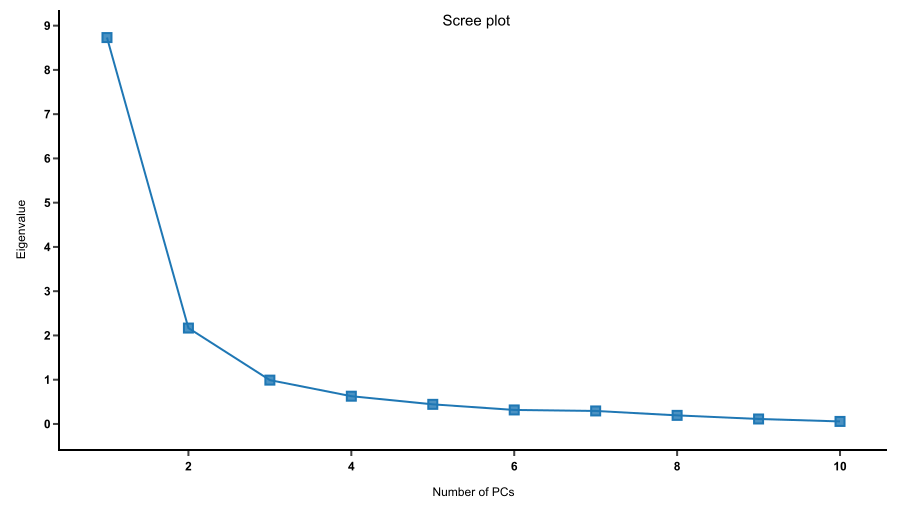
\includegraphics[width=250pt, height=170pt]{Scree}
		\captionof{figure}{Scree plot}
	\end{minipage}
\end{center}

\item Интерпретируем столько компонент, сколько можем.
\end{enumerate}

\section{Оптимизация в АГК в терминах ковариационных матриц}
	Напомним,  что $\mathbb{Y}=\mathbb{X}^\mathrm{T}$, где $\mathbb{X}$ --- матрица данных.


\begin{proposition}
	 Задача $\Arrowvert \mathbb{Y}-\widetilde{\mathbb{Y}}\Arrowvert \to \min \limits_{\widetilde{\mathbb{Y}}:~\rnk\widetilde{\mathbb{Y}}\le r}$ эквивалентна задаче $\Arrowvert \mathbb{Y}\mathbb{Y}^\mathrm{T}-\widetilde{\mathbb{Y}}\widetilde{\mathbb{Y}}^\mathrm{T}\Arrowvert \to \min \limits_{\widetilde{\mathbb{Y}}:~\rnk\widetilde{\mathbb{Y}}\le r}$.
Решение этой задачи $\widetilde{\mathbb{Y}}^*$ строится как сумма собственных троек, соответствующих первым $r$ главным компонентам.
\end{proposition}

Если матрица центрирована, то задача $\Arrowvert \mathbb{Y}\mathbb{Y}^\mathrm{T}-\widetilde{\mathbb{Y}}\widetilde{\mathbb{Y}}^\mathrm{T}\Arrowvert \to \min \limits_{\widetilde{\mathbb{Y}}:~\rnk\widetilde{\mathbb{Y}}\le r}$ эквивалентна следующей задаче:
\begin{equation*}
\Arrowvert \mathbb{S}-\widetilde{\mathbb{S}}\Arrowvert \to \min \limits_{\widetilde{\mathbb{S}}:~\rnk\widetilde{\mathbb{S}}\le r},
\end{equation*}
где $\mathbb{S}$ --- ковариационная матрица для наших данных, а $\widetilde{\mathbb{S}}$ --- какая-то ковариационная матрица (симметричная, неотрицательно определенная).

%\end{document}
\newpage
\chapter{Факторный анализ\\ (EFA --- exploratory factor analysis)}

\section{Модель в факторном анализе}

Главное отличие факторного анализа от анализа главных компонент --- это наличие модели в факторном анализе.

Пусть $\bm\xi=(\xi_1,\ldots,\xi_p)^\mathrm{T} \in \mathbb{R}^p$, $\bm\eta=(\eta_1,\ldots,\eta_r)^\mathrm{T}\in\mathbb{R}^r$, $r<p$. Предполагаем, что $\mathbb{E}\xi_i=0,$ $\mathbb{E}\eta_i=0, ~\mathbb{D}\eta_i=1,$ $\eta_i$ и $\eta_j$ некоррелированы.
Пусть $\mathbb{F}_r=[F_1:\ldots:F_r]\in\mathbb{R}^{p\times r}$.
(Помните --- у нас есть $p$ старых признаков и мы строим новых. Новые $r$ признаков будут в каком-то смысле самыми лучшими.)

Итак, \emph{модель в факторном анализе}: $$\bm\xi=\mathbb{F}_r\bm\eta+\bm\varepsilon,$$ где  ковариационная матрица $\text{Cov}\,\bm\varepsilon=\diag(\sigma_1^2,\ldots,\sigma_p^2)$ диагональная, $\bm\eta$ и $\bm\varepsilon$ некоррелированы. Случайному вектору $\bm\xi$ соответствует матрица данных $\mathbb{X}^\mathrm{T}$ (признаки, которые мы наблюдаем), а $\bm\eta$ соответствует $\mathbb{V}_r^\mathrm{T}$ (скрытые признаки, которые мы не наблюдаем). Получаем соотношение $$\mathbb{X}=\mathbb{V}_r\mathbb{F}_r^\mathrm{T}+\mathbb{E}.$$ Перед нами стоит задача выявить эти скрытые признаки (задача факторного анализа). Причем, даже нет цели найти значения факторов. Цель --- найти их смысл.

Заметим, что модель очень похожа на то, что можно получить с помощью АГК:
$$\mathbb{X}=\mathbb{V}_{1,r}\mathbb{F}_{1,r}^\mathrm{T}+\mathbb{V}_{r+1,d}\mathbb{F}_{r+1,d}^\mathrm{T},$$
но есть разница (увидим позже).

Модель можно переписать в следующем виде:
\begin{equation*} \Sigma = \text{Cov}(\xi)=\text{Cov}(\mathbb{F}_r\eta)+\text{Cov}(\bm\varepsilon)=\mathbb{F}_r\mathbb{F}_r^\mathbb{T}+\Psi,
\end{equation*}
где $\Psi=\diag(\sigma_1^2,\ldots,\sigma_p^2), ~\rnk \mathbb{F}_r\mathbb{F}_r^\mathbb{T}\le r. $ Тогда данные --- это выборочная ковариационная матрица.

Вообще, факторный анализ всегда делается на основе стандартизованных данных. Т.е. всегда мы получаем модель корреляционной матрицы. Тогда $f_{ij}=\rho(\xi_i,\eta_j)$ и матрица факторных нагрузок выглядит следующим образом:

\begin{table}[H]
	\centering
	\begin{tabular}{c|ccc}
      &	$\eta_1$ & $\ldots$ & $\eta_r$ \\
		\hline
	$\xi_1$	&      $f_{11}$    &   $\ldots$ & $f_{1r}$             \\
		$\vdots$	&     $\vdots$    &   & $\vdots$            \\
		$\xi_p$	&      $f_{p1}$    &   $\ldots$ & $f_{pr}$             \\
	\end{tabular}
\end{table}

Модель:
\begin{equation*}
\xi_1=f_{11}\eta_1+\ldots+f_{1i}\eta_i+\ldots+f_{1r}\eta_r+(\varepsilon_1+0\varepsilon_2+\ldots+0\varepsilon_p)
\end{equation*}
\begin{equation*}
\xi_2=f_{21}\eta_1+\ldots+f_{2i}\eta_i+\ldots+f_{2r}\eta_r+(0\varepsilon_1+\varepsilon_2 +\ldots+0\varepsilon_p)
\end{equation*}
\begin{equation*}
\ldots
\end{equation*}
\begin{equation*}
\xi_p=f_{p1}\eta_1+\ldots+f_{pi}\eta_i+\ldots+f_{pr}\eta_r+(0\varepsilon_1+0\varepsilon_2+\ldots+\varepsilon_p)
\end{equation*}

Мы предполагаем, что в каждом столбце (и строчке) перед $\varepsilon_i$ только один из коэффициентов не равен нулю, а среди $f_{ij}$, $i=1,\ldots,p$, хотя бы два не равны нулю.

\section{Общности и уникальности}

В этом пункте введем понятие общности и уникальности признаков.

Обозначим $\bm\xi'= \mathbb{F}_r \bm\eta$, тогда $\bm\xi = \bm\xi'+\bm\varepsilon$. То есть $\bm\xi'$ --- это та часть данных, которая описывается факторами. Предполагаем, что $\textsf{D}\xi_i=1,$ $\textsf{D}\varepsilon_i=\sigma_i^2,$ тогда $\textsf{D}\xi_i'=\textsf{D}\xi_i-\textsf{D}\varepsilon_i= 1-\sigma_i^2.$

Можно заметить, что $\text{Cov}(\xi_i, \xi_j)=\text{Cov}(\xi_i'+\varepsilon_i, \xi_j'+\varepsilon_j) = \text{Cov}(\xi_i', \xi_j')$, так как остальные слагаемые обнуляются из-за некоррелированности. Получаем, что $\text{Cov}(\xi_i', \xi_j')=\rho_{ij}$. Также известно, что ковариационная матрица $\bm\xi'$ равна $\text{Cov} (\bm\xi') = \mathbb{F}_r \text{Cov}(\bm\eta) \mathbb{F}_r^\mathrm{T} = \mathbb{F}_r\mathbb{F}_r^\mathrm{T}.$

Тогда
\begin{equation*}
\mathbb{F}_r\mathbb{F}_r^\mathrm{T} = \text{Cov} (\bm\xi') =
\left(\begin{matrix}
1-\sigma_1^2 & \ldots & \rho_{1p} \\
\vdots & \ddots & \vdots \\
\rho_{p1} & \ldots & 1-\sigma_p^2 \\
\end{matrix}  \right).
\end{equation*}

Мы получили, что

\begin{equation*}
1 = \textsf{D}\xi_i = \textsf{D}\xi_i'+\textsf{D}\varepsilon_i = \underbrace{(1-\sigma_i^2)}_{\substack{\text{commonality}, \\  \text{общность признака}}} + \underbrace{\sigma_i^2}_{\substack{\text{uniquence}, \\  \text{уникальность}}}.
\end{equation*}


\begin{remark}
 Общность является множественным коэффициентом корреляции:
 \begin{equation*}
\underbrace{\textsf{D}\xi_i'}_{\text{общность}} = (\mathbb{F}_r\mathbb{F}_r^\mathrm{T})_{ii} = f_{i1}^2+f_{i2}^2+\ldots+f_{ir}^2 = \sum\limits_{j=1}^r f_{ij}^2 = \sum \limits_{j=1}^r (\rho(\xi_i,\eta_j))^2 = R^2(\xi_i | \eta_1,\ldots, \eta_r),
 \end{equation*}
 т.к. $\eta_i$ и $\eta_j$ некоррелированы.
\end{remark}

Таким образом, общность --- это то, что описывается факторами, а уникальность признака --- то, что не описывается факторами.

\section{Корректность поставленной задачи}
Теперь посмотрим, корректно ли поставлена задача?

Во-первых, напомним, что в матрице $\mathbb{F}$ не может быть такого столбца, где только один элемент не равен нулю, то есть это факторы, соответствующие хотя бы двум признакам. Случайные величины из вектора $\bm\varepsilon$ в каком-то смысле тоже факторы, но каждый из них соответствует только одному признаку. Факторный анализ ищет общие факторы.

Определим $\widetilde{\mathbb{F}}_r=\mathbb{F}_r\mathbb{W},$ где $\mathbb{W} \in \mathbb{R}^{r\times r}$ --- ортогональная матрица. Тогда
\begin{equation*} \widetilde{\mathbb{F}}_r\widetilde{\mathbb{F}}_r^\mathrm{T}=\mathbb{F}_r\mathbb{W}\mathbb{W}^\mathrm{T}\mathbb{F}_r^\mathrm{T}=\mathbb{F}_r\mathbb{F}_r^\mathrm{T},
\end{equation*}
то есть решение не единственно, и любое вращение --- тоже решение. Необходимо добавить ограничения, чтобы как-то зафиксировать решение. Матрица $\mathbb{W}$ содержит $\frac{r(r-1)}{2}$ параметров (известный факт --- ортогональную матрицу размерности $r\times r$ можно задать таким количеством параметров). Следовательно, для однозначности модели необходимо добавить столько же ограничений, чтобы убрать свободу.
\begin{example}
	Пусть $\mathbb{S}$ --- выборочная ковариационная матрица.
	
	 Тогда ограничение: $\mathbb{F}_r^\mathrm{T}\mathbb{S}\mathbb{F}_r$ --- диагональная матрица $r\times r$. Тут $\frac{r(r-1)}{2}$ ограничений (из-за симметричности число ограничений равно числу нулей под диагональю матрицы).
\end{example}

Теперь посчитаем число параметров в модели $\Sigma=\mathbb{F}_r\mathbb{F}_r^\mathbb{T}+\Psi$. Тут
\begin{equation*}
\underbrace{pr}_{\text{для }\mathbb{F}_r}+\underbrace{p}_{\text{для }\Psi}-\underbrace{\frac{r(r-1)}{2}}_{\text{вычитаем число ограничений}}
\end{equation*}
параметров с учетом ограничений.

Модель задается $\frac{p(p+1)}{2}$ равенствами. Тогда нужно требовать, чтобы число параметров не превосходило число уравнений, то есть
\begin{equation*}
pr+p-\frac{r(r-1)}{2}\le \frac{p(p+1)}{2}.
\end{equation*}
Если записать это неравенство в другом виде, то получим
\begin{equation*}
\frac{(p-r)^2-(p+r)}{2}\ge 0.
\end{equation*}

\section{Задача оценивания параметров}
Теперь можем перейти к задаче оценивания параметров. Можно оценивать несколькими методами.

\subsection{Метод наименьших квадратов (OLS)}

Пусть $\mathbb{S}=\{s_{ij}\}_{i,j=1}^p$ --- выборочная ковариационная матрица.

Решаем задачу $\Arrowvert \mathbb{S}-\widetilde{\mathbb{S}}\Arrowvert_2^2 \to \min\limits_{\widetilde{\mathbb{S}}:~ \widetilde{\mathbb{S}}=\widetilde{\mathbb{F}}_r\widetilde{\mathbb{F}}_r^\mathrm{T}+\widetilde{\Psi}}$, что эквивалентно задаче
\begin{equation*}
\sum\limits_{i,j=1}^p (s_{ij}-\widetilde{s}_{ij})^2\to \min\limits_{\widetilde{\mathbb{S}}:~ \widetilde{\mathbb{S}}=\widetilde{\mathbb{F}}_r\widetilde{\mathbb{F}}_r^\mathrm{T}+\widetilde{\Psi}}
\end{equation*}

\textbf{Алгоритм MINRES} (OLS для ковариационной матрицы):
\begin{enumerate}
	\item Рассматриваем не всю матрицу, а ее часть, и решаем следующую задачу:\footnote{Матрицу $\Psi$ убрали, т.к. она диагональна, а мы суммируем по всем $i\ne j$.}
	\begin{equation*}
	\sum\limits_{i\ne j} \underbrace{(s_{ij}-\widetilde{s}_{ij})^2}_{\text{residuals}}\to \min\limits_{\widetilde{\mathbb{S}}:~ \widetilde{\mathbb{S}}=\widetilde{\mathbb{F}}_r\widetilde{\mathbb{F}}_r^\mathrm{T}}.
	\end{equation*}
    \item Находим $\hat{\mathbb{F}}_r$.%\footnote{Находим какую-то симметричную, неотрицательно определенную матрицу ранга $r$, а потом с учетом ограничений однозначно находим $\mathbb{F}_r$.}
    \item $\left( \begin{matrix}
    	\sigma_1^2 \\
    	\vdots \\
    	\sigma_p^2
    	\end{matrix} \right) = \underbrace{\left( \begin{matrix}
    	1 \\
    	\vdots \\
    	1
    	\end{matrix} \right)}_{\text{Диагональ } \mathbb{S}} -~ (\text{Диагональ }\widetilde{\mathbb{F}}_r\widetilde{\mathbb{F}}_r^\mathrm{T})$
\end{enumerate}

\subsection{Взвешенный метод наименьших квадратов (WLS)}

Решается задача
\begin{equation*}
\sum\limits_{i,j=1}^p \frac{(s_{ij}-\widetilde{s}_{ij})^2}{\widehat{\sigma}_i^2 \widehat{\sigma}_j^2}\to \min\limits_{\widetilde{\mathbb{S}}:~ \widetilde{\mathbb{S}}=\widetilde{\mathbb{F}}_r\widetilde{\mathbb{F}}_r^\mathrm{T}+\widetilde{\Psi}}
\end{equation*}

Получаем, что чем меньше уникальность, тем больше вес слагаемого.

\subsection{Метод максимального правдоподобия (MLE)}
Выписывается распределение ковариационной матрицы данных в модели факторного анализа
и находятся оценки параметров ее максимизацией. Результат примерно такой же, как в WLS.


\section{Разница между АГК и факторным анализом}

Первое отличие между факторным анализом и анализом главных компонент заключается в наличии модели в факторном анализе.

Второе отличие состоит в том, что у АГК и факторного анализа разные оптимизационные задачи. \textbf{Задача факторного анализа}:

\begin{equation*}
\sum\limits_{i\ne j} (s_{ij}-\widetilde{s}_{ij})^2\to \min\limits_{\widetilde{\mathbb{S}}:~ \widetilde{\mathbb{S}}=\widetilde{\mathbb{F}}_r\widetilde{\mathbb{F}}_r^\mathrm{T}},
\end{equation*}
 где минимизируется сумма по всем элементам, кроме диагональных, $\widetilde{\mathbb{S}}$ --- симметричная, неотрицательно определенная матрица ранга, не превосходящего $r$.

\textbf{Задача в анализе главных компонент}:
\begin{equation*}
\sum\limits_{i,j} (s_{ij}-\widetilde{s}_{ij})^2 \to \min\limits_{\widetilde{\mathbb{S}}:~ \widetilde{\mathbb{S}}=\widetilde{\mathbb{F}}_r\widetilde{\mathbb{F}}_r^\mathrm{T}},
\end{equation*}
минимизируется сумма по всем элементам, $\widetilde{\mathbb{S}}$ --- симметричная, неотрицательно определенная матрица ранга, не превосходящего $r$.

Таким образом, цель факторного анализа --- как можно лучше воспроизвести ковариации. В анализе главных компонент стоит аппроксимизационная задача, и АГК не решает именно задачу факторного анализа, хотя все равно используется для поиска факторов на практике.

Есть еще третье различие, которое рассмотрим ниже --- в факторном анализе порядок факторов не важен (в АГК они упорядочены по вкладу), а важен их смысл.

\section{Проверка гипотез}

\subsection{Проверка значимости модели}
Рассмотрим гипотезу $H_0:~ \Sigma=\mathbb{F}_r\mathbb{F}_r^\mathrm{T}+\Psi$ о том, что $\Sigma$ действительно имеет такой вид. Статистика критерия
\begin{equation*}
t=(n-1-\frac{2p+4r-5}{6})\log \frac{\overbrace{|\widehat{\mathbb{F}}_r\widehat{\mathbb{F}}_r^\mathrm{T}+\widehat{\Psi}|}^{\text{То, что ожидаем}}}{\underbrace{|\mathbb{S}|}_{\text{То, что есть}}} \sim \chi^2(\frac{(p-r)^2-(p+r)}{2})
\end{equation*}
(в нормальной модели).

Идеальное значение равно $0$ (логарифм будет равен нулю, если данные идеально соответствуют гипотезе, критическая область справа).

\subsection{Тест сферичности Бартлетта}
Для начала необходимо проверить, есть ли вообще структура. Гипотеза о том, что общей структуры нет: $H_0: ~ \Sigma=\mathbb{I}_{p\times p}$ (единичная матрица).

Тест сферичности Бартлетта: статистика критерия
\begin{equation*}
t=(n-1-\frac{2p-5}{6})(-\log |\mathbb{S}|) \sim \chi^2(\frac{p(p-1)}{2})
\end{equation*}
(в нормальной модели).

Для выбора порядка модели можно применять информационные критерии AIC, BIC (в нормальной модели) --- подход со штрафом за число параметров. Можно промоделировать, посчитать вклады (несколько раз) и строить доверительный интервал.

\newpage
\section{Ортогональные вращения}

Имеем $\mathbb{F}_r=\{f_{ij}\}=\{\rho(\xi_i,\eta_j)\}$. Мы интерпретируем признаки в факторном анализе, смотря на элементы $f_{ij}$ (как исходные признаки выражаются через факторы). Нам хотелось бы, чтобы матрица $\mathbb{F}_r$ имела простую структуру (то есть чтобы в ней было много нулей).

Заметим, что если $\mathbb{F}_r$ --- решение, то вращение $\widetilde{\mathbb{F}}_r=\mathbb{F}_r\mathbb{W}$ --- тоже решение, только будут другие корреляции между исходными признаками и факторами, так как меняется $\mathbb{F}_r$. (Матрица вращения $\mathbb{W}$ ортогональна.)

На выборочном языке: $\mathbb{X}'$ --- та часть исходных данных, которая описывается факторами (соответствует $\bm\xi'=\mathbb{F}_r\bm\eta$).
\begin{equation*}
\mathbb{X}'=\mathbb{V}\mathbb{F}^\mathrm{T}_r=\underbrace{\mathbb{V}\mathbb{W}}_{\widetilde{\mathbb{V}}}\underbrace{\mathbb{W}^\mathrm{T}\mathbb{F}^\mathrm{T}_r}_{\widetilde{\mathbb{F}}_r},
\end{equation*}
$\widetilde{\mathbb{V}}$ --- новые факторы, $\widetilde{\mathbb{F}}_r$ --- новые факторные нагрузки. Хотелось бы найти такую $\mathbb{W},$ чтобы интерпретация была как можно проще.

\begin{example}
	Пусть у нас какие-то признаки отвечают за знание математики, а другие за знание физики.
	\begin{center}
	\begin{minipage}{0.7\linewidth}
		\centering
\vspace{-0.5in}
		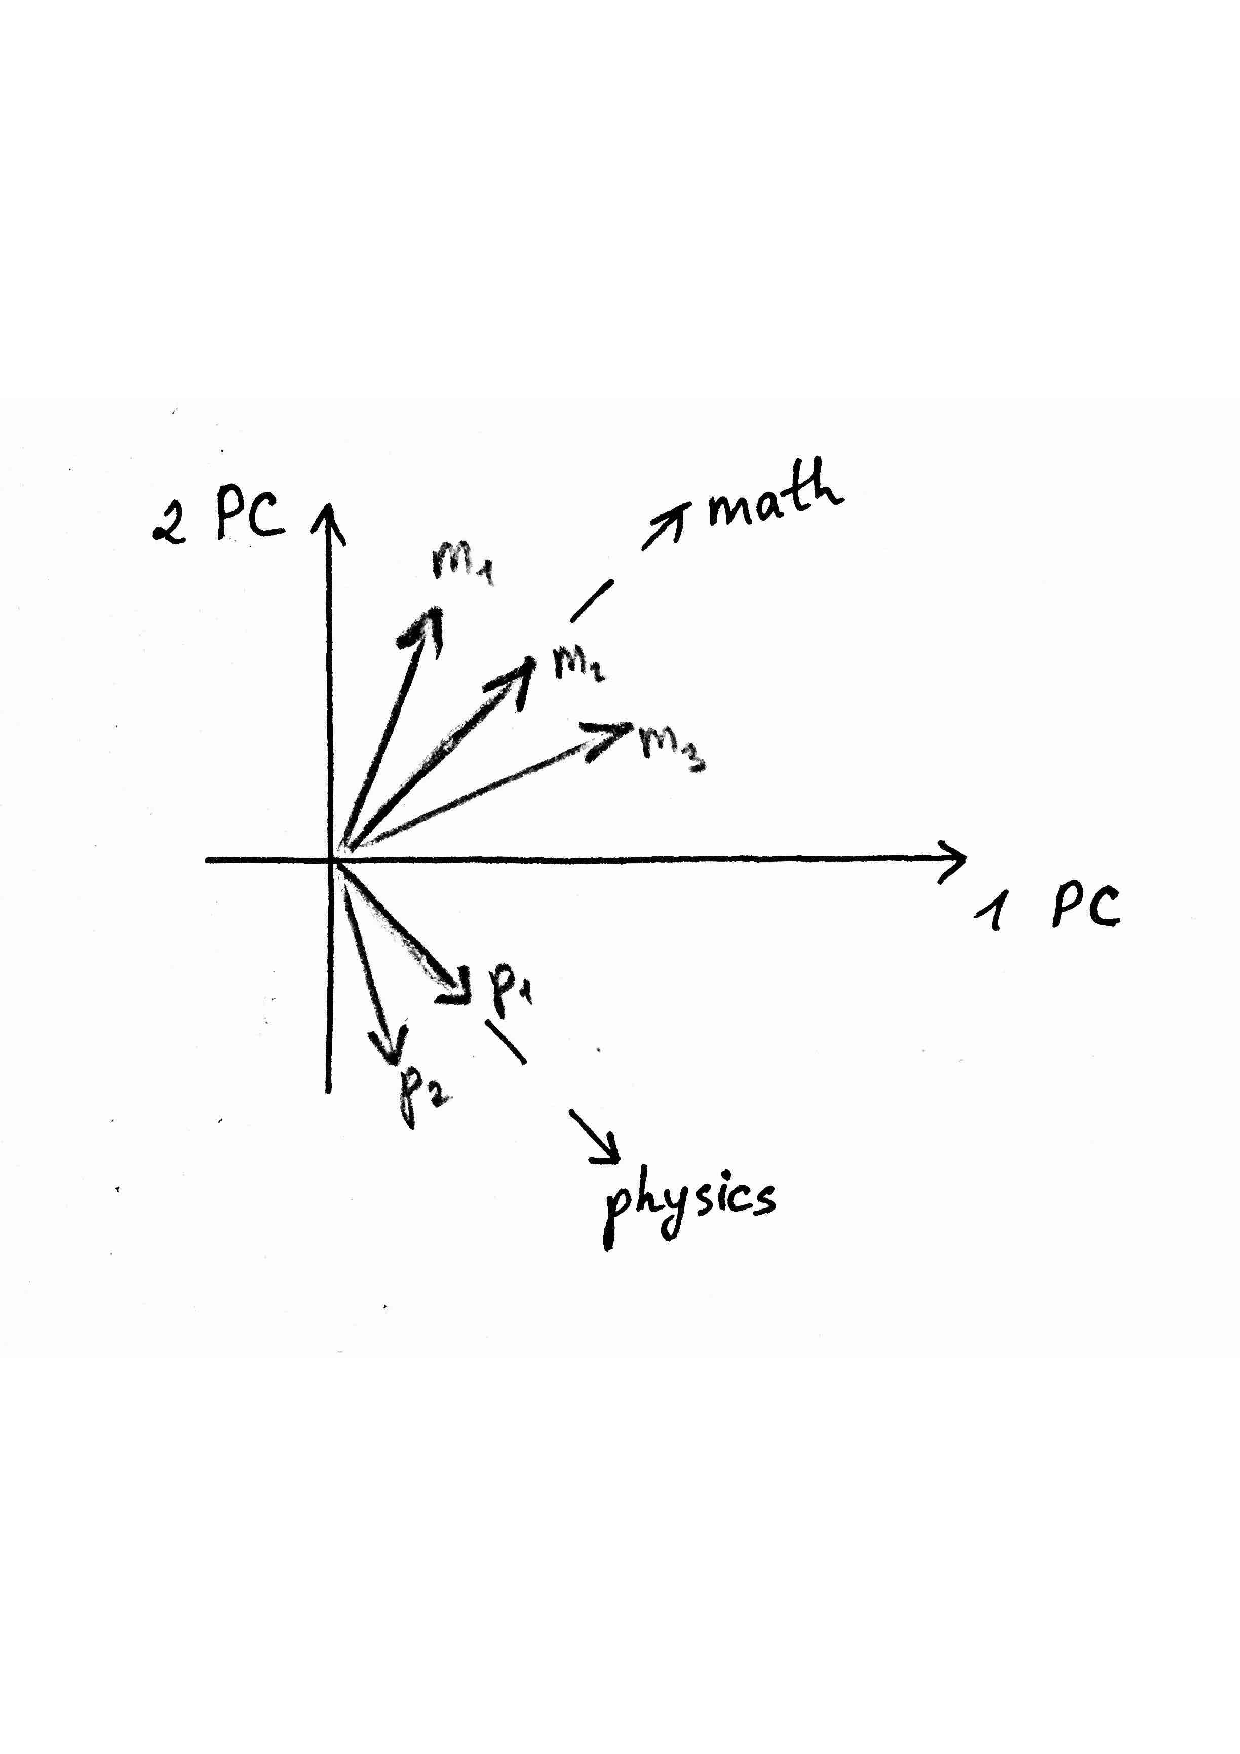
\includegraphics[width=230pt, height=210pt]{p12}
\vspace{-0.7in}
		\captionof{figure}{Вращение в факторном анализе}
	\end{minipage}
\end{center}

Мы можем повернуть данные так, что у нас одна ось совпадет, к примеру, с признаком $m_2$, а другая с признаком $p_1$. Тогда интерпретировать станет проще.
\end{example}


\textbf{Метод вращений Varimax}:
Хотим получить более понятную интерпретацию, для этого нам будет удобно, если в каждом столбце матрицы $\mathbb{F}_r$ было как можно больше нулей. Задача выглядит следующим образом:
\begin{equation*}
\sum\limits_{j=1}^r \big[\frac{1}{p}\sum\limits_{i=1}^p(\widetilde{f}_{ij}^2)^2-(\frac{1}{p}\sum\limits_{i=1}^p\widetilde{f}_{ij}^2)^2\big] \to \max\limits_{\mathbb{W}:~ \widetilde{\mathbb{F}}_r=\mathbb{F}_r\mathbb{W} },
\end{equation*}
где мы рассматриваем $f_{ij}^2$, так как $f_{ij}$ могут быть отрицательны, и считаем разброс значений $f_{ij}^2$, $i=1,\ldots,p$, как выборочную дисперсию, так как чем больше разброс, тем больше шансов, что значения будут разными, т.е. маленькие (почти нулевые) и большие.

\textbf{На выборочном языке:} $\mathbb{V}=[V_1:\ldots:V_r], ~ V_1,\ldots,V_r\in\mathbb{R}^n$ --- факторные вектора. На выборочном языке $\bm\xi$ переходит в $\mathbb{X}\in\mathbb{R}^{n\times p}$, $\bm\xi'$ переходит в $\mathbb{X}'\in\mathbb{R}^{n\times p}$, $\bm\eta$ (соответствует факторам) переходит в $\mathbb{V}\in\mathbb{R}^{n\times r}$. Тогда $\mathbb{F}\bm\eta$ соответствует $\mathbb{V}\mathbb{F}^\mathrm{T}$.

Поворачиваем факторы: $\widetilde{\bm\eta}=\mathbb{W}\bm\eta$ --- факторы после вращения, $\widetilde{\mathbb{F}}=\mathbb{F}\mathbb{W}^{-1},$ где $\mathbb{W}\in\mathbb{R}^{r\times r}$ --- матрица поворота. Что означает на языке векторов то, что мы поворачиваем факторы? Это значит, что $\widetilde{\mathbb{V}}=\mathbb{V}\mathbb{W}\in\mathbb{R}^{n\times r}$.

Идея: мы хотим, чтобы $\mathbb{F}\bm\eta=\widetilde{\mathbb{F}}\widetilde{\bm\eta}$ (то есть $\bm\xi'$ не должно меняться). И действительно,
\begin{equation*}
\widetilde{\mathbb{F}}\widetilde{\bm\eta}=\mathbb{F}\mathbb{W}^{-1}\mathbb{W}\bm\eta=\mathbb{F}\bm\eta,
\end{equation*}
мы поменяли факторные веса и получили то же самое (условно можно сказать, что в одну сторону поворачиваем факторы и в другую сторону поворачиваем $\mathbb{F}$).

В случае ортогональных вращений: $\mathbb{W}^{-1}=\mathbb{W}^{\mathrm{T}}$ и тоже является матрицей поворота.


\section{Косоугольные вращения}

Если мы допускаем косоугольные вращения, то, вообще говоря, $\mathbb{W}^{-1}\ne\mathbb{W}^{\mathrm{T}}$. Мы хотим, чтобы новые факторы после вращения были по-прежнему нормированы (то есть дисперсия была равна 1 на языке случайных величин). Мы предполагаем, что все центрировано. Тогда
\begin{equation*}
\text{Cov}(\widetilde{\bm\eta})=\textsf{E}\widetilde{\bm\eta}\widetilde{\bm\eta}^\mathrm{T} = \textsf{E}(\mathbb{W}\bm\eta\bm\eta^\mathrm{T}\mathbb{W}^\mathrm{T}) = \mathbb{W} \underbrace{\text{Cov}\,\bm\eta}_{\mathbb{I}_{r\times r}} \mathbb{W}^\mathrm{T} = \mathbb{W}\mathbb{W}^\mathrm{T},
\end{equation*}
будем требовать, чтобы на диагонали этой матрицы стояли единицы.

\begin{remark}
	Необходимо проверять, чтобы в корреляционной матрице новых факторов были не очень большие по модулю корреляции, так как чем больше корреляции между новыми признаками, тем более подозрительный результат.
\end{remark}

Интерпретация после косоугольных вращений уже становится непонятна.

\newpage
\section{Факторная структура и факторный паттерн}

Введем определения для двух матриц.

\begin{definition}
	Факторная структура (factor structure) --- это матрица корреляций исходных признаков с новыми, то есть $\Phi = \{\rho(\xi_i,\widetilde{\eta}_j)\}_{i=1,j=1}^{p,r}$.
\end{definition}

\begin{definition}
	Факторный паттерн (factor pattern, factor loadings) --- это матрица $\widetilde{\mathbb{F}}$, коэффициенты линейной комбинации в $\bm\xi'=\widetilde{\mathbb{F}}\widetilde{\bm\eta}$ (коэффициенты линейной комбинации, с которыми исходные признаки выражаются через новые).
\end{definition}

\begin{proposition}
	В случае ортогональных вращений факторная структура совпадает с факторным паттерном.
\end{proposition}
\begin{proof}
Распишем, чему равно $\Phi$:
\begin{equation*}
\Phi = \text{Cov}(\bm\xi,\widetilde{\bm\eta})=\textsf{E}(\bm\xi'\widetilde{\bm\eta}^\mathrm{T}) = \textsf{E}(\widetilde{\mathbb{F}}\widetilde{\bm\eta}\widetilde{\bm\eta}^\mathrm{T}) = \widetilde{\mathbb{F}}\text{Cov}(\widetilde{\bm\eta}) =  \widetilde{\mathbb{F}}\mathbb{W}\mathbb{W}^\mathrm{T}.
\end{equation*}
В случае ортогональных вращений $\mathbb{W}^{-1}=\mathbb{W}^{\mathrm{T}}$, следовательно $\Phi = \widetilde{\mathbb{F}}\underbrace{\mathbb{W}\mathbb{W}^\mathrm{T}}_{\mathbb{I}_{r \times r}} = \widetilde{\mathbb{F}}$.
\end{proof}

\section{Методы нахождения факторных значений}

Перейдем на выборочный язык. $\mathbb{X}=\mathbb{V}\mathbb{F}^\mathrm{T}+\mathcal{E}.$ Пусть мы уже оценили $\mathbb{F}$. Возникает вопрос --- как найти $\mathbb{V}$ (factor scores)? Есть несколько методов.
\begin{enumerate}
	\item (OLS) Распишем по индивидам $Y_i \in \mathbb{R}^p$, получим $n$ уравнений
	\begin{equation*}
	Y_i = \mathbb{F} \left( \begin{matrix}
	v_{i1} \\
	\vdots \\
	v_{ir}
	 \end{matrix} \right) + \mathcal{E}_i, ~~~ i=1,\ldots,n
	\end{equation*}
	Факторные значения для $i$-ого индивида можно найти по методу наименьших квадратов, тогда решение выглядит следующим образом:
	\begin{equation*}
	(v_{i1},\ldots,v_{ir})^\mathrm{T} = (\mathbb{F}^\mathrm{T}\mathbb{F})^{-1}\mathbb{F}^\mathrm{T}Y_i.
	\end{equation*}
	
	\item (Метод Бартлетта (WLS)) Пусть $\Psi = \diag(\sigma_1^2, \ldots, \sigma_p^2)$ --- диагональная матрица, в которой на диагонали стоят уникальности. Тогда решение:
	\begin{equation*}
	(v_{i1},\ldots,v_{ir})^\mathrm{T} = (\mathbb{F}^\mathrm{T}\Psi^{-1}\mathbb{F})^{-1}\mathbb{F}^\mathrm{T}\Psi^{-1}Y_i.
	\end{equation*}
	
	\item (Regression method) В нормальной модели, основываясь на ОМП,
		\begin{equation*}
	(v_{i1},\ldots,v_{ir})^\mathrm{T} = \mathbb{F}^\mathrm{T}\mathbb{S}^{-1}Y_i.
	\end{equation*}
	
\end{enumerate}



\end{document} 